\documentclass[aspectratio=169,10pt]{beamer}
\usepackage[T1]{fontenc}
\usepackage{lmodern}
\usepackage{amsmath,amssymb,bm,booktabs}
\usepackage{graphicx,tikz,attachfile2}
\usetikzlibrary{arrows.meta,positioning,calc}
\definecolor{ink}{HTML}{203348}
\definecolor{accent}{HTML}{007C91}
\definecolor{warm}{HTML}{BD6339}
\definecolor{muted}{HTML}{58697B}
\definecolor{pale}{HTML}{EDF5F7}
\setbeamercolor{normal text}{fg=ink,bg=white}
\setbeamercolor{frametitle}{fg=ink,bg=white}
\setbeamercolor{structure}{fg=accent}
\setbeamercolor{block title}{fg=accent,bg=pale}
\setbeamercolor{block body}{fg=ink,bg=pale}
\setbeamercolor{takeaway}{fg=ink,bg=pale}
\setbeamerfont{frametitle}{size=\Large,series=\bfseries}
\setbeamerfont{block title}{size=\normalsize,series=\bfseries}
\setbeamersize{text margin left=0.65cm,text margin right=0.65cm}
\setbeamertemplate{navigation symbols}{}
\setbeamertemplate{itemize item}{\color{accent}\small$\bullet$}
\setbeamertemplate{footline}{\leavevmode\hbox{\begin{beamercolorbox}[wd=.87\paperwidth,ht=2.8ex,dp=1.3ex,leftskip=.65cm]{normal text}\color{muted}\scriptsize Physical diffusion models with fast hidden units\hspace{1em}|\hspace{1em}PI discussion, 11 Nov 2026\end{beamercolorbox}\begin{beamercolorbox}[wd=.13\paperwidth,ht=2.8ex,dp=1.3ex,rightskip=.65cm plus1fil]{normal text}\hfill\scriptsize\insertframenumber\end{beamercolorbox}}}
\setbeamertemplate{frametitle}{\vspace{0.16cm}\insertframetitle\par\vspace{0.07cm}{\color{accent}\rule{\textwidth}{0.6pt}}}
\title{Physical diffusion models with fast hidden units}
\date{11 November 2026}
\hypersetup{colorlinks=true,urlcolor=accent,linkcolor=accent,pdftitle={Physical diffusion models with fast hidden units},pdfsubject={PI discussion: theory, MNIST samples, parameter schedules and conditional Potts probabilities}}
\pdfstringdefDisableCommands{\def\translate#1{#1}}
\ifdefined\shownotes\setbeameroption{show only notes}\else\setbeameroption{hide notes}\fi
\newcommand{\vx}{\bm{x}}
\newcommand{\Ev}{E^{\mathrm v}}
\newcommand{\grad}{\nabla}
\newcommand{\takeaway}[1]{\begin{beamercolorbox}[sep=.16cm,wd=\textwidth]{takeaway}\small #1\end{beamercolorbox}}
\newcommand{\source}[1]{\par\vspace{.08cm}{\fontsize{6.5}{8}\selectfont\color{muted}#1\par}}
\newcommand{\timeheaders}{\par\noindent\hspace*{.13724\linewidth}\makebox[.14617\linewidth]{$s=0$}\makebox[.14617\linewidth]{$1.26$}\makebox[.14617\linewidth]{$2.53$}\makebox[.14617\linewidth]{$3.79$}\makebox[.14617\linewidth]{$5$}\par\vspace{.06cm}}
\newcommand{\statefigure}[3]{\timeheaders\centering\includegraphics[page=2,trim={14 #2 14 #3},clip,width=.94\textwidth]{assets/parameter_evolution_draft.pdf}\par\vspace{.12cm}\takeaway{State #1. Shared $W$ and $Q$ colour scales across all shown states and times.}\source{Saved coefficients; $s=5-t$. Initial digit associations describe the initialization clusters.}}

\begin{document}

\begin{frame}[plain]
  \vspace{.4cm}
  {\color{accent}\large PI discussion\par}
  \vspace{.45cm}
  {\fontsize{26}{30}\selectfont\bfseries Physical diffusion models\par with fast hidden units\par}
  \vspace{.5cm}
  {\large From a local energy model to global digit structure\par}
  \vspace{.65cm}
  \begin{beamercolorbox}[sep=.3cm,wd=.93\textwidth]{takeaway}
    Slow visible oscillators\quad$+$\quad fast hidden statistics\par\vspace{.16cm}
    Local training\quad$\longrightarrow$\quad open-loop generation
  \end{beamercolorbox}
  \vfill
  {\color{muted}Theory, all-ten-digit MNIST samples, learned schedules and a trajectory movie\par\vspace{.15cm}11 November 2026}
  \note{Suggested length: about 20 minutes for the main slides, with detailed coupling maps in backup. The objective is to explain exactly what the current model implements and what the saved numerical results establish. These are simulations, not an experimental hardware demonstration. The primary diagnostic run is Potts1536 with local Ising units.}
\end{frame}

\begin{frame}{The idea: train local interactions, replay a schedule}
  \begin{columns}[c,onlytextwidth]
    \column{.64\textwidth}
      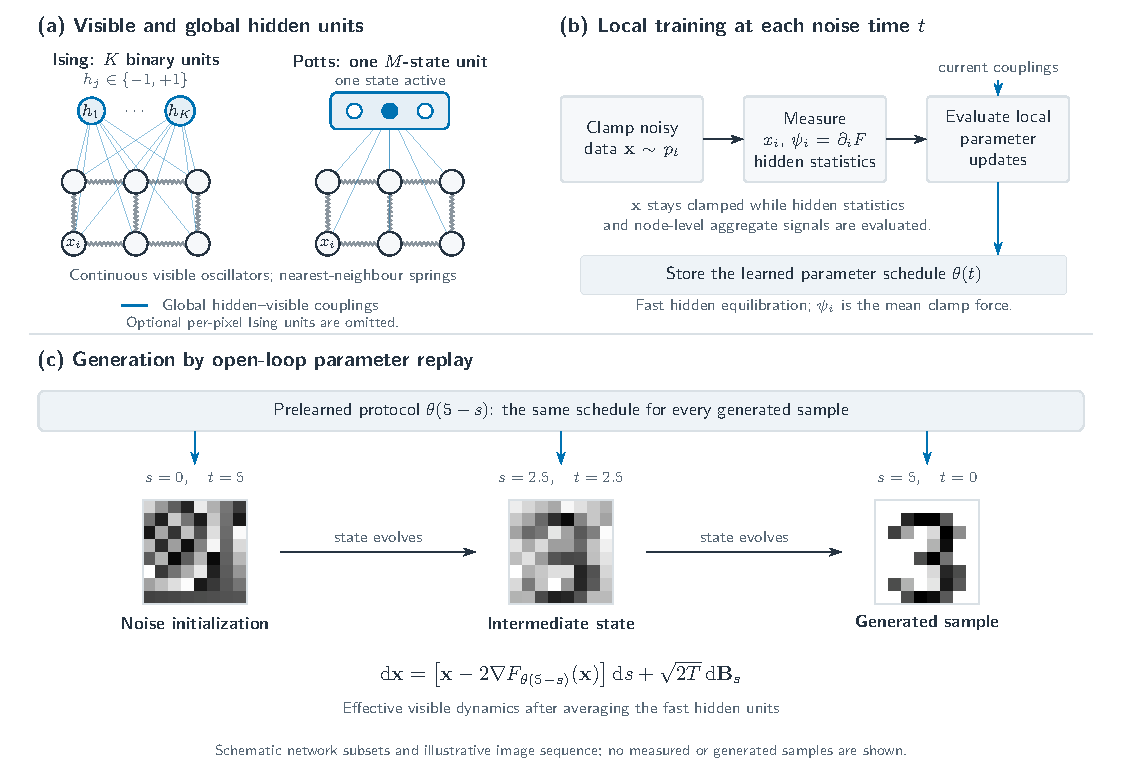
\includegraphics[width=\linewidth]{assets/conceptual_draft.pdf}
    \column{.33\textwidth}
      \textbf{Architecture}\par Continuous pixels with neighbour springs and global hidden coupling.
      \vspace{.35cm}\par\textbf{Training}\par Clamp noisy data; use mean forces and conditional hidden statistics.
      \vspace{.35cm}\par\textbf{Generation}\par Replay the learned parameters as a function of time.
      \vspace{.3cm}\par{\small\color{muted}Overview is schematic. Optional local Ising units are omitted here.}
  \end{columns}
  \note{Use the existing overview to introduce the three stages. Its image sequence is a drawing, not generated samples. The current numerical results also include one additional local hidden Ising spin per pixel; the next slide makes that architecture explicit. Open loop means the parameter schedule is prescribed; it does not mean the physical force is independent of the current state.}
\end{frame}

\begin{frame}{The Potts run we are actually inspecting}
  \begin{columns}[c,onlytextwidth]
    \column{.49\textwidth}
    \centering
    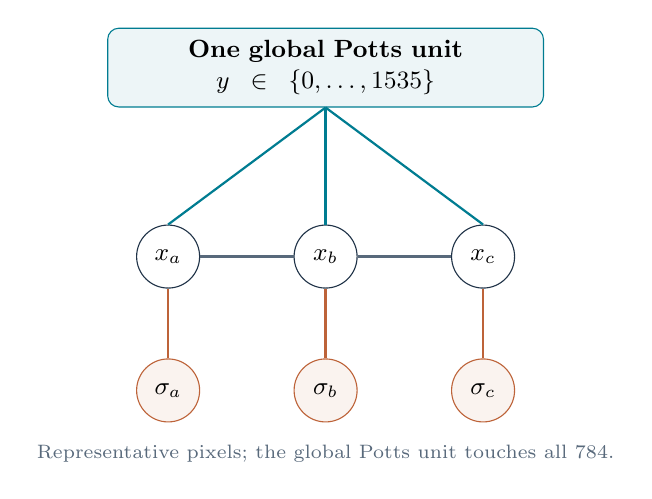
\begin{tikzpicture}[x=1cm,y=1cm,>=Stealth,every node/.style={font=\small}]
      \node[draw=accent,fill=pale,rounded corners,text width=5.3cm,align=center,minimum height=1cm] (p) at (0,2.4) {\textbf{One global Potts unit}\\$y\in\{0,\ldots,1535\}$};
      \foreach \x/\name in {-2/a,0/b,2/c}{
        \node[circle,draw=ink,fill=white,minimum size=.8cm] (v\name) at (\x,0) {$x_{\name}$};
        \node[circle,draw=warm,fill=warm!8,minimum size=.8cm] (h\name) at (\x,-1.7) {$\sigma_{\name}$};
        \draw[accent,thick] (p.south) -- (v\name.north);
        \draw[warm,thick] (v\name.south) -- (h\name.north);
      }
      \draw[thick,muted] (va) -- (vb);\draw[thick,muted] (vb) -- (vc);
      \node[align=center,text=muted,font=\scriptsize] at (0,-2.5) {Representative pixels; the global Potts unit touches all 784.};
    \end{tikzpicture}
    \column{.47\textwidth}
      \begin{itemize}\setlength\itemsep{.22cm}
        \item $784$ continuous visible oscillators, $28\times28$ pixels.
        \item One shared Potts label with $1536$ states.
        \item $784$ additional hidden Ising spins, one per pixel.
        \item Up to eight visible neighbours; $2970$ distinct spring edges.
        \item Quartic on-site potentials; quadratic Potts coupling enabled.
      \end{itemize}
      \vspace{.2cm}\takeaway{All ten digits. Training uses exact conditional hidden statistics.}
  \end{columns}
  \note{This is the completed all-ten-digit Potts1536 run with quadratic hidden coupling, local Ising spins, quartic visible potentials and eight-neighbour springs. Potts1536 means one unit with 1536 mutually exclusive states, not 1536 Potts units. Local spins are separate from the continuous visible oscillators. Interior pixels have eight neighbours; boundary pixels have fewer. The code marginalizes both types of hidden unit.}
\end{frame}

\begin{frame}{Eliminating hidden states gives a free energy}
  \setlength{\abovedisplayskip}{4pt}\setlength{\belowdisplayskip}{4pt}
  At one fixed diffusion time, let $E(\vx,y)$ be the joint energy.
  \vspace{.15cm}
  \begin{align*}
    Z_h(\vx)&=\sum_y e^{-E(\vx,y)/T},
    &p(y\mid\vx)&=\frac{e^{-E(\vx,y)/T}}{Z_h(\vx)},\\[.15cm]
    F(\vx)&=-T\log Z_h(\vx),
    &p_\theta(\vx)&\propto e^{-F(\vx)/T}.
  \end{align*}
  \begin{block}{The identity that connects statistics to mechanics}
    \centering\vspace{.1cm}$\displaystyle\boxed{-\grad F(\vx)=\big\langle-\grad_{\vx} E(\vx,y)\big\rangle_{y\mid\vx}}$\par\vspace{.1cm}
  \end{block}
  \vspace{.18cm}\par
  $F(\vx)=\langle E\rangle_{y\mid\vx}-T S(y\mid\vx)$ includes the hidden-state entropy.
  \vspace{.2cm}\par
  \takeaway{The static marginal is exact. Using this mean force dynamically requires fast hidden equilibration.}
  \note{For continuous hidden variables the sum becomes an integral. All derivatives are at fixed temperature and fixed parameters. Differentiating the logarithm of the conditional partition sum produces the normalized Boltzmann weights. Free energy is not merely the arithmetic mean of state energies: hidden entropy contributes. Physical force is minus the gradient; the mean clamp force is plus the gradient.}
\end{frame}

\begin{frame}{Fast hopping can produce a smooth average force}
  \begin{columns}[c,onlytextwidth]
    \column{.57\textwidth}
      \[E_m(\vx)=\Ev(\vx)-a_m(\vx),\qquad \bm f_m=-\grad E_m.\]
      \begin{align*}
        -\grad F
        &=-\grad\Ev+T\grad\log\sum_m e^{a_m/T}\\[.16cm]
        &=-\grad\Ev+\sum_m p_m\grad a_m\\[.16cm]
        &=\sum_m p_m\bm f_m.
      \end{align*}
    \column{.39\textwidth}
      \begin{block}{For example}
        Spend $70\%$ of the time in state 1 and $30\%$ in state 2:
        \[\overline{\bm f}=0.7\bm f_1+0.3\bm f_2.\]
      \end{block}
      \small Hidden mixing must be fast compared with visible motion \emph{and} changes in the parameter schedule.
  \end{columns}
  \vspace{.3cm}
  \takeaway{The simulation evaluates the average directly. It contains no discrete hidden jumps or switching rates.}
  \note{A physical hidden unit occupies one state at a time and hops stochastically. In an ergodic process, the equilibrium probabilities become dwell-time fractions over a sufficiently long window. The averaging window must still be short on the visible and schedule timescales. The same equilibrium probabilities can occur for fast or slow kinetics. Since the probabilities depend on x, averaging the forces does not imply a blurry average image. The movie later shows probability competition, not measured jump events.}
\end{frame}

\begin{frame}{Potts: one label selects a state-dependent landscape}
  \begin{columns}[t,onlytextwidth]
    \column{.60\textwidth}
      \begin{align*}
        E_{\rm eff}(\vx,y=m)&=G(\vx)-a_m(\vx),\\
        a_m(\vx)&=b_m+\bm W_m\!\cdot\!\vx+\bm Q_m\!\cdot\!\vx^2,\\
        p_m(\vx)&=\frac{e^{a_m/T}}{\sum_k e^{a_k/T}},\\[.16cm]
        \bm f_{\rm Potts}&=\sum_m p_m(\vx)\bigl(\bm W_m+2\bm Q_m\circ\vx\bigr).
      \end{align*}
      \small $G=\Ev+F_{\rm local}$ includes the local Ising contribution when present.
    \column{.36\textwidth}
      \textbf{$W_m$: linear tilt}\par Changes the preferred visible configuration.
      \vspace{.25cm}\par\textbf{$Q_m$: stiffness change}\par It is not the covariance itself.
      \vspace{.25cm}\par\textbf{$b_m$: energy offset}\par Changes relative occupation, not spatial position.
  \end{columns}
  \vspace{.28cm}
  \takeaway{A mixture of $M$ conditional visible distributions. They are Gaussian only for a quadratic common energy.}
  \note{At an actual hidden state m only row m of W and Q and entry m of b enter the energy. The effective energy here is already a partial free energy because the local Ising spins have been marginalized. Marginalizing the Potts unit then sums over all its labels. The current common energy contains quartic visible potentials and local Ising free energies, so the components are generally non-Gaussian. W is not directly the mean image and Q is not directly a covariance. A backup slide gives the Gaussian special case. Initial k-means labels are diagnostics, not constraints restricting a state to a digit class.}
\end{frame}

\begin{frame}{Ising: binary hidden units can act in combination}
  \begin{columns}[t,onlytextwidth]
    \column{.60\textwidth}
      \begin{align*}
        h_j&\in\{-1,+1\},\quad j=1,\ldots,K,\\
        E_{\rm eff}(\vx,\bm h)&=G(\vx)-\sum_j h_j a_j(\vx),\\
        F(\vx)&=G(\vx)-T\sum_j\log\!\left[2\cosh\frac{a_j(\vx)}{T}\right],\\
        \langle h_j\mid\vx\rangle&=\tanh\!\frac{a_j(\vx)}{T},\\
        \bm f_{\rm Ising}&=\sum_j\tanh(a_j/T)\,\grad a_j.
      \end{align*}
    \column{.36\textwidth}
      \begin{block}{Global Ising architecture}
        Each spin couples to all pixels. $K$ binary spins give $2^K$ joint configurations.
      \end{block}
      \begin{block}{Additional local spins}
        One per pixel: $a_i^{\rm loc}=c_i+w_i x_i$.
        \[f_i^{\rm loc}=w_i\tanh\frac{c_i+w_i x_i}{T}.\]
      \end{block}
  \end{columns}
  \note{Global Ising and global Potts are alternative architectures; local Ising units can accompany either. Multiple global Ising spins can contribute simultaneously, unlike one mutually exclusive Potts label. They are conditionally independent at fixed $x$ because there are no hidden-hidden couplings; after marginalizing $x$ they need not be independent. The field $a_j$ can include the same $Q_j x^2$ term. $2^K$ is a count of joint configurations, not a claim of $2^K$ learned distinct useful digits.}
\end{frame}

\begin{frame}{Training uses clamped noisy data and hidden statistics}
  At each noise time $t$, fit $F_\theta$ to the score of $p_t$:
  \[\mathcal J_T(\theta)=\mathbb E_{\vx\sim p_t}
    \left[-\frac{\Delta F_\theta}{T}+\frac{\|\grad F_\theta\|^2}{2T^2}\right].\]
  \begin{columns}[t,onlytextwidth]
    \column{.49\textwidth}
      \begin{block}{Visible parameters: $\Ev=\sum_k\theta_k\phi_k$}
        \[\partial_{\theta_k}\mathcal J_T=
          \left\langle-\frac{\Delta\phi_k}{T}
          +\frac{\grad\phi_k\cdot\bm\psi}{T^2}\right\rangle,\]
        where $\bm\psi=\grad F$ is the mean clamp force.
      \end{block}
    \column{.47\textwidth}
      \begin{block}{Hidden parameters}
        Updates combine pixel signals, conditional occupations/moments, current couplings and state-level aggregates.
        \vspace{.18cm}\par No free-running negative phase is required.
      \end{block}
  \end{columns}
  \takeaway{The all-ten-digit results here use exact conditional statistics. Finite-read hardware training is a separate test.}
  \note{This is a local rule in the sense developed in the theory note: synapse updates use node/pixel quantities and aggregates, but the hidden updates still depend on the current weights. Do not call them parameter-independent Hebbian updates. Earlier smaller experiments study finite-sample readouts and bias corrections, but the all-ten-digit examples in this presentation use exact conditional statistics. This slide motivates the paper's training claim without implying an experimental hardware implementation.}
\end{frame}

\begin{frame}{Generation replays the learned parameters open loop}
  \begin{align*}
    \text{Forward noise:}\quad &d\vx=-\vx\,dt+\sqrt{2T}\,d\bm B_t,\\[.25cm]
    \text{Generation:}\quad &s=5-t,\\[-.05cm]
    &\boxed{d\vx=\bigl[\vx-2\grad F_{\theta(5-s)}(\vx)\bigr]ds
       +\sqrt{2T}\,d\bm B_s.}
  \end{align*}
  \vspace{.25cm}
  \begin{itemize}\setlength\itemsep{.2cm}
    \item One learned schedule $\theta(t)$, linearly interpolated between 100 time slices.
    \item The same schedule for every generated image; no training during generation.
    \item Hidden probabilities respond to the evolving $\vx$ through the couplings.
  \end{itemize}
  \vspace{.15cm}\takeaway{The effective potential for generation is $2F-\|\vx\|^2/2$; physical realization must reproduce that force.}
  \note{T=0.02 and the forward horizon is 5. The explicit x term and the factor two distinguish the reverse-SDE drift from the energy force -grad F. Doubling all hidden couplings at fixed hidden temperature does not simply double their free energy. Exact physical constructions include two hidden replicas at temperature T or an appropriate amplification of back-action; see the theory note. The saved parameter plots show the generation-time schedule, not optimizer iteration history.}
\end{frame}

\begin{frame}{All ten digits: saved samples from both architectures}
  \begin{columns}[t,onlytextwidth]
    \column{.49\textwidth}\centering
      \textbf{One Potts unit, $M=1536$}\par\vspace{.08cm}
      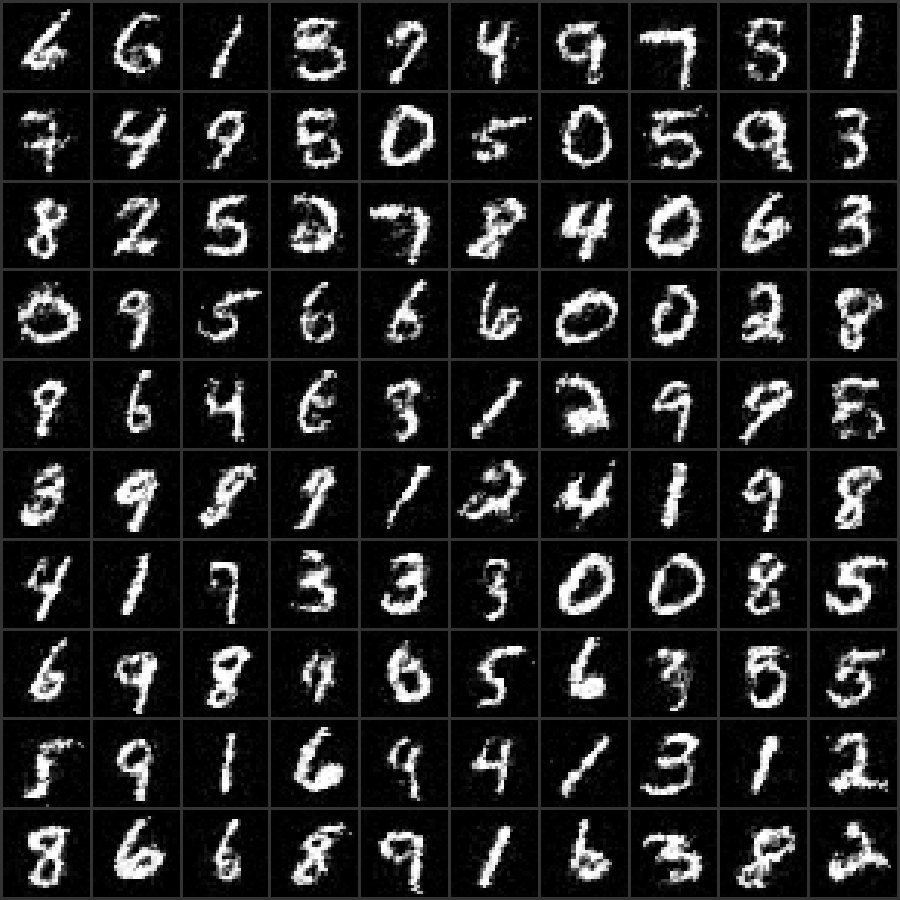
\includegraphics[height=5.35cm]{assets/sample_potts.pdf}
    \column{.49\textwidth}\centering
      \textbf{Global Ising, $K=784$}\par\vspace{.08cm}
      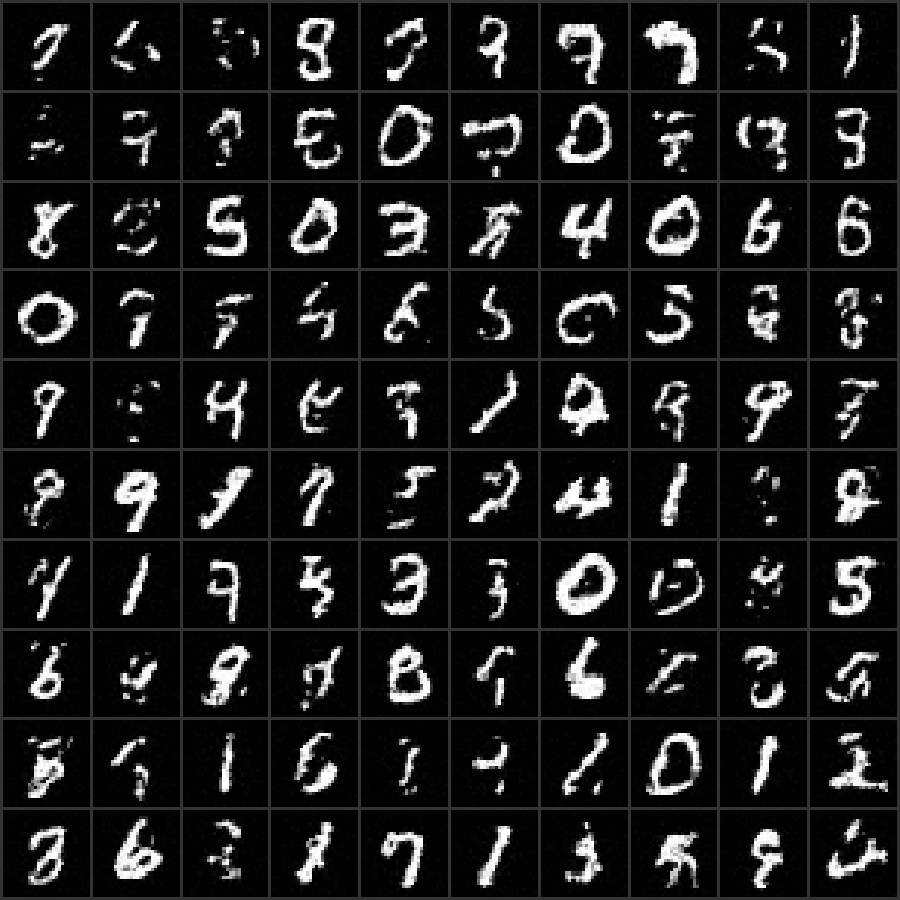
\includegraphics[height=5.35cm]{assets/sample_ising.pdf}
  \end{columns}
  \source{First 100 images of each saved base-2000 sample set, unfiltered and in saved order. Both include local Ising units and eight-neighbour visible springs. These are examples, not a controlled ranking.}
  \note{Both panels are rendered from already saved samples; no new training or sampling is performed for this slide. Each panel uses the first 100 images from its own base-2000 set with fixed display normalization. Counts differ between the global hidden architectures, so this is not a matched-capacity comparison. Call these completed examples, not the best possible Potts or Ising model. Exact source configs and hashes are in the sample-gallery provenance JSON in the assets folder.}
\end{frame}

\begin{frame}{Visible parameters develop strong spatial structure}
  \begin{columns}[c,onlytextwidth]
    \column{.76\textwidth}\centering
      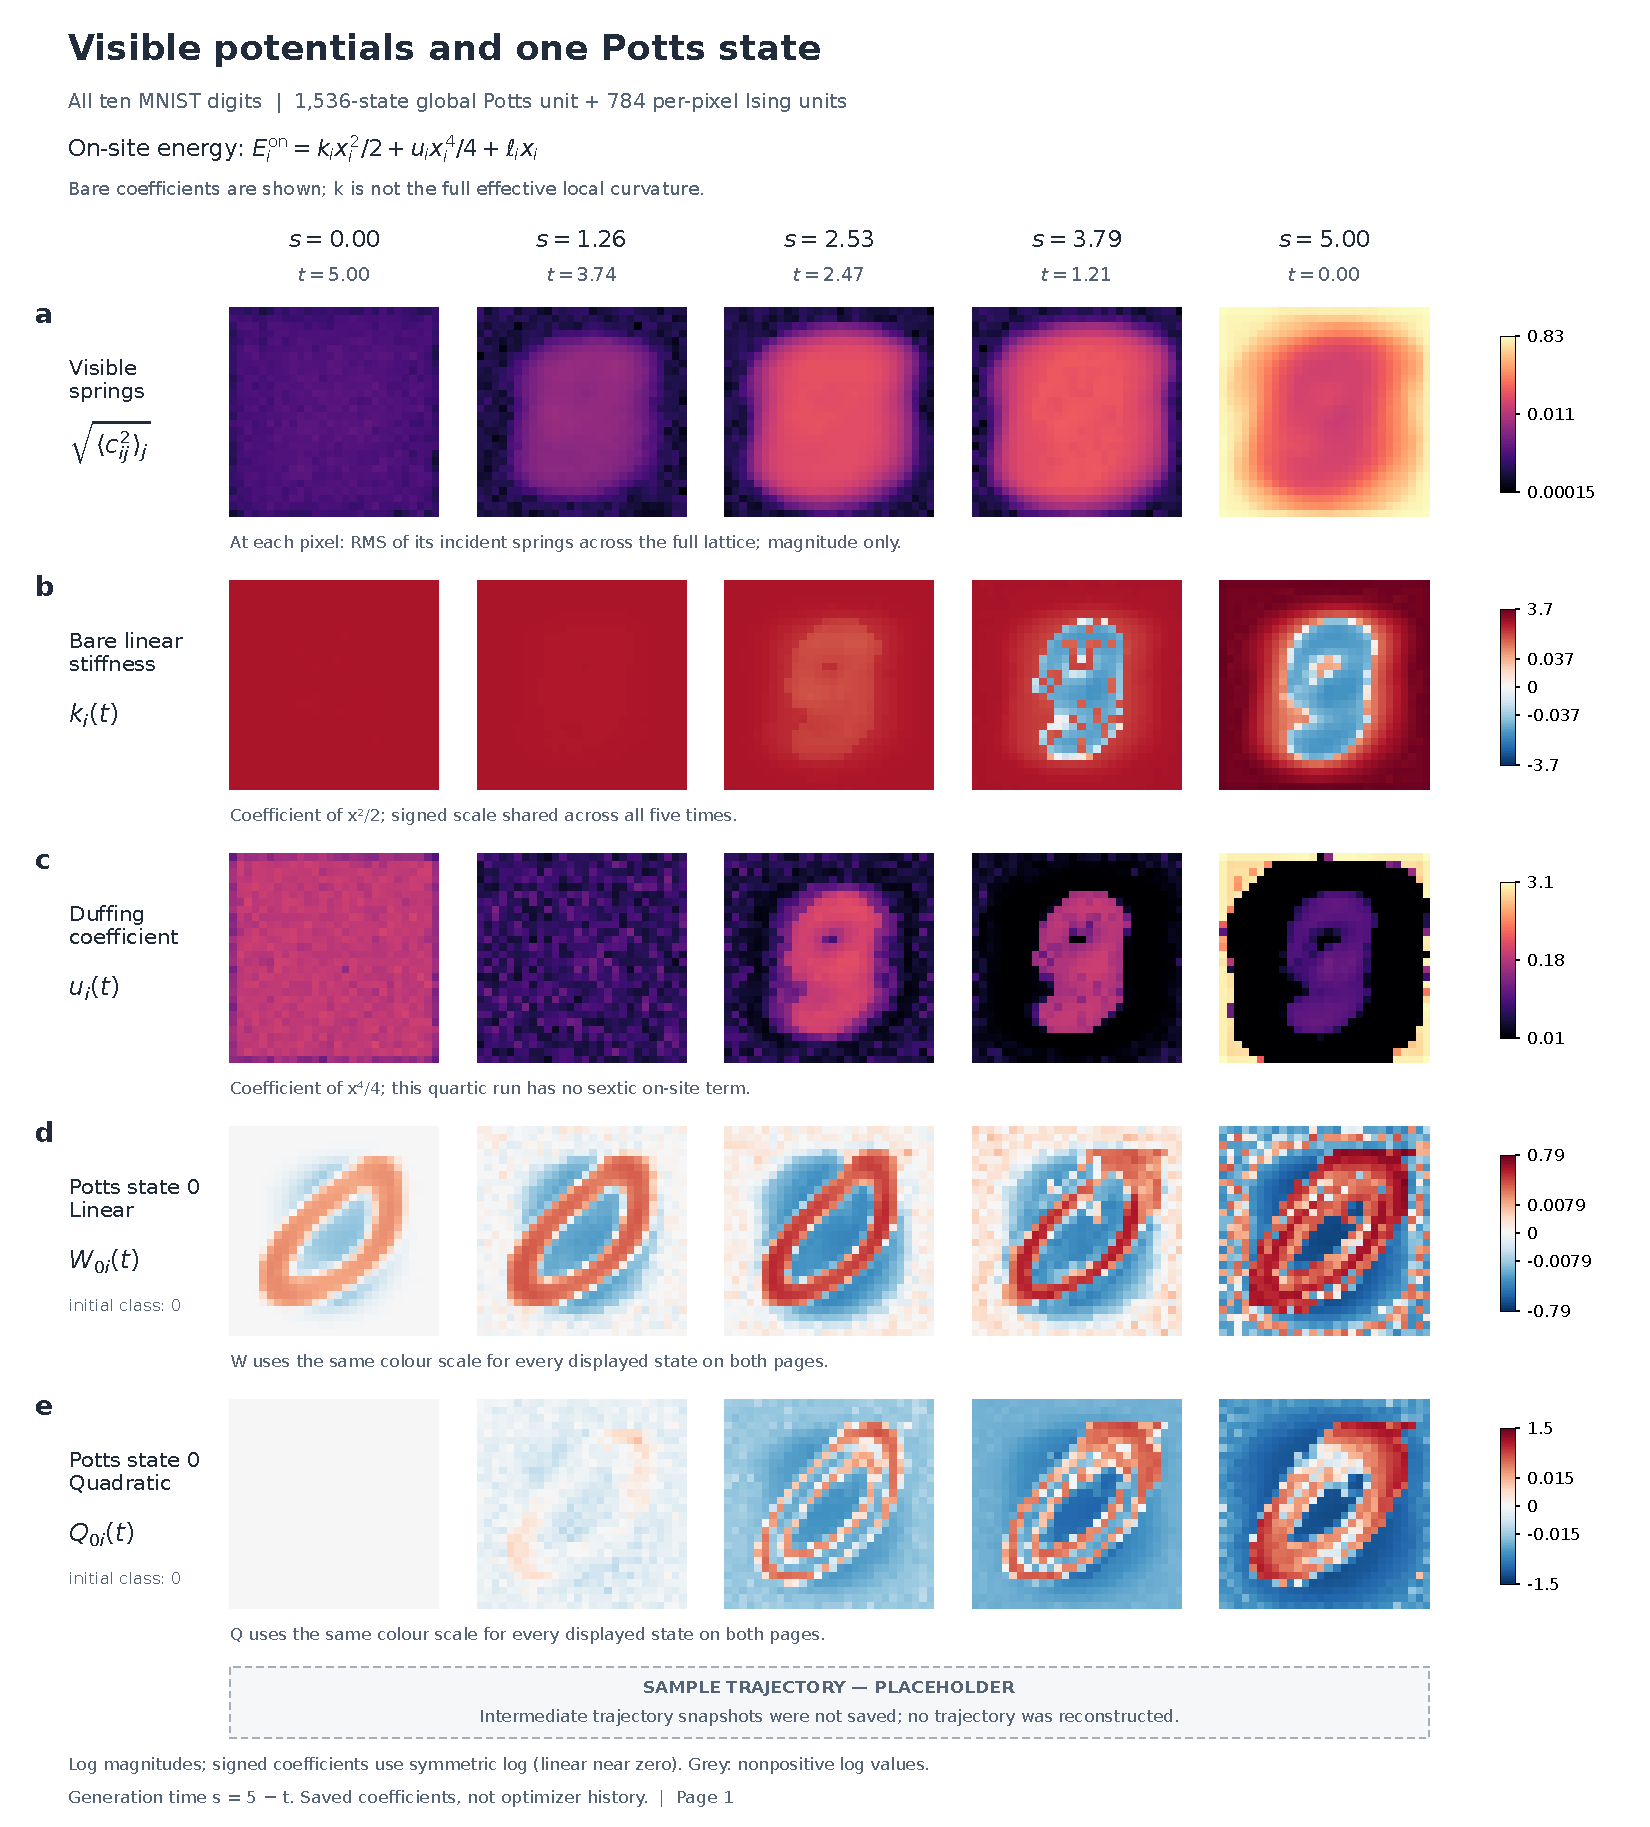
\includegraphics[page=1,trim={14 343.96 14 108},clip,width=\linewidth]{assets/parameter_evolution_draft.pdf}
    \column{.21\textwidth}
      \small\textbf{Top: springs}\par RMS of incident $c_{ij}$.
      \vspace{.28cm}\par\textbf{Middle: $k_i$}\par Bare coefficient of $x_i^2/2$.
      \vspace{.28cm}\par\textbf{Bottom: $u_i$}\par Duffing coefficient of $x_i^4/4$.
      \vspace{.28cm}\par\color{muted}Log magnitudes; signed $k_i$ uses symmetric log.
  \end{columns}
  \source{Potts1536 diagnostic run. Columns follow generation time $s=5-t$. Colour scales are shared across time within each row.}
  \note{These are learned parameter schedules, not curves of learning progress. The on-site energy is $k_i x_i^2/2 + u_i x_i^4/4 + \ell_i x_i$. The linear stiffness is bare: visible springs, $3u_i x_i^2$, and hidden curvature affect the full local response. Spring maps summarize RMS magnitude of incident edges, not signed coefficients. Border structure should not be interpreted as springs pinning absolute intensity; spring forces vanish for any uniform configuration.}
\end{frame}

\begin{frame}{One Potts state's coupling pattern evolves with time}
  \timeheaders
  \centering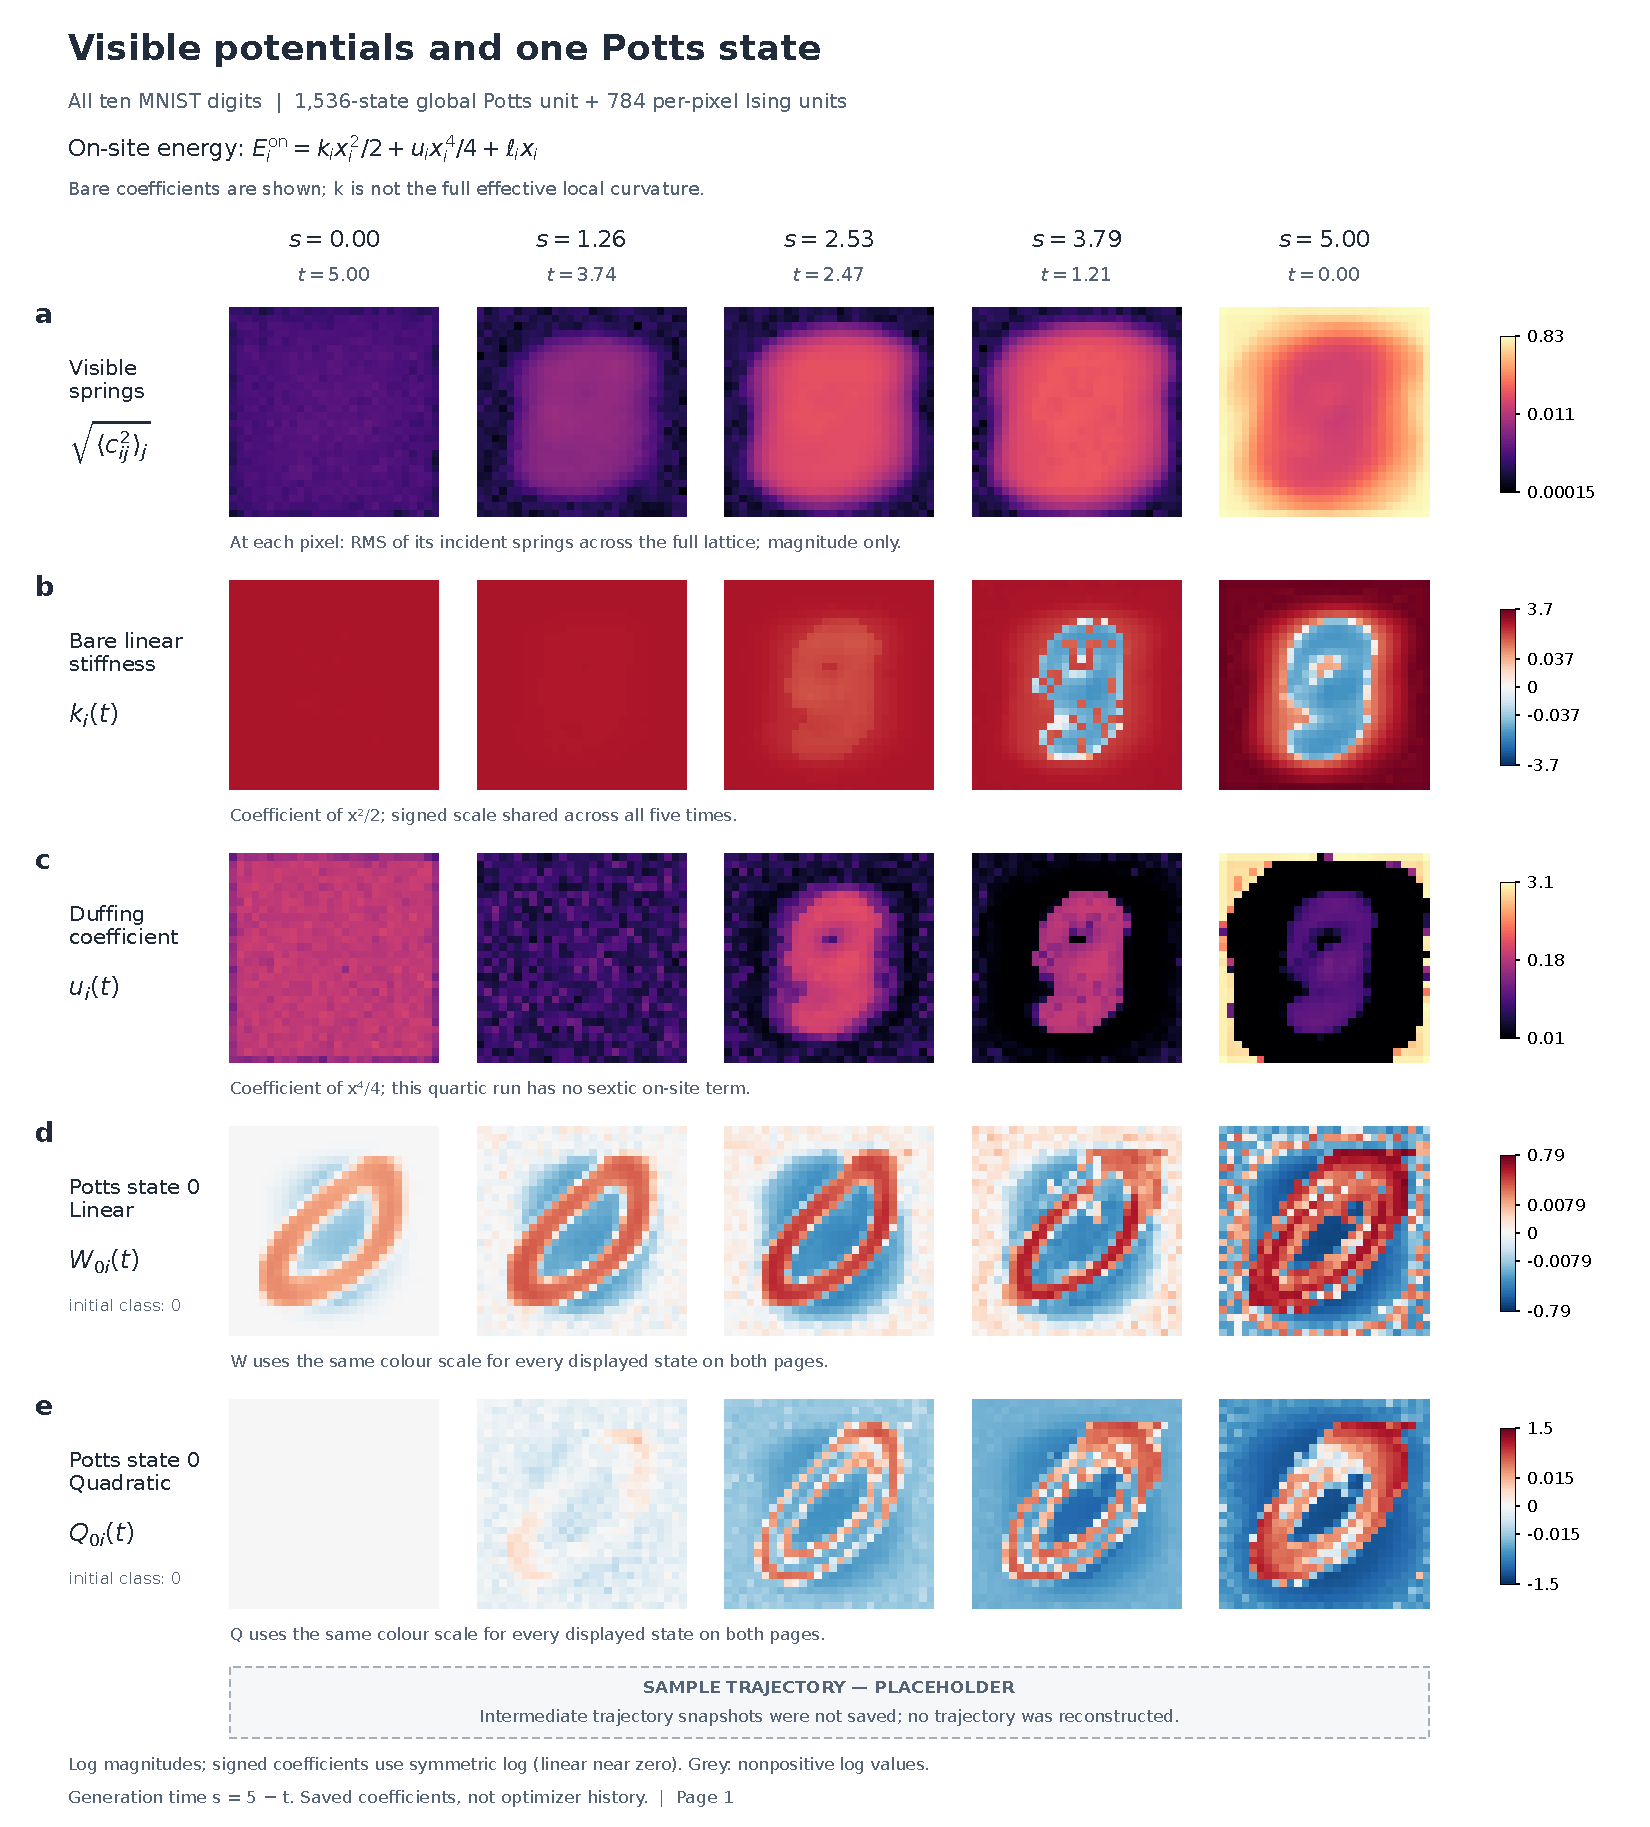
\includegraphics[page=1,trim={14 83 14 533},clip,width=.94\textwidth]{assets/parameter_evolution_draft.pdf}
  \vspace{.12cm}
  \takeaway{$W_{0i}$ supplies a linear field; $Q_{0i}$ changes local stiffness. The pattern resembles a prototype.}
  \source{State 0, whose initial cluster majority label is 0. Raw coefficients; common symmetric-log scales across states and times.}
  \note{Only state 0 is displayed on this slide, with its linear and quadratic couplings to all visible pixels. This is not the mean of a Gaussian component. The state index was fixed rather than chosen for high final occupancy or sample quality. The same state is followed through the schedule. The previous placeholder trajectory panel was omitted from this crop because an actual trajectory movie is now available.}
\end{frame}

\begin{frame}{Other Potts states carry different spatial patterns}
  \centering
  \begin{tabular}{c c c c}
    &\textbf{State 1}&\textbf{State 2}&\textbf{State 4}\\
    &\small initial group 6&\small initial group 2&\small initial group 9\\[.08cm]
    $W_{mi}$&\includegraphics[page=2,trim={582 717.4 14 145},clip,width=3.8cm]{assets/parameter_evolution_draft.pdf}&\includegraphics[page=2,trim={582 455.4 14 407},clip,width=3.8cm]{assets/parameter_evolution_draft.pdf}&\includegraphics[page=2,trim={582 193.4 14 669},clip,width=3.8cm]{assets/parameter_evolution_draft.pdf}\\[.08cm]
    $Q_{mi}$&\includegraphics[page=2,trim={582 585.4 14 277},clip,width=3.8cm]{assets/parameter_evolution_draft.pdf}&\includegraphics[page=2,trim={582 323.4 14 539},clip,width=3.8cm]{assets/parameter_evolution_draft.pdf}&\includegraphics[page=2,trim={582 61.4 14 801},clip,width=3.8cm]{assets/parameter_evolution_draft.pdf}
  \end{tabular}
  \vspace{.15cm}\takeaway{Final-time couplings, $s=5$. Initial cluster labels are approximate associations, not measured final class purity.}
  \source{Crops of the existing parameter figure. Each coefficient family uses the same scale for all states. Full schedules are in backup.}
  \note{States 1,2,4 were chosen earlier to include different initial cluster majority labels (6,2,9), not because of a measured quality score. These are visual patterns in coupling fields; we should not claim every state stores one pure class, nor that digit labels restrict possible transitions. Colour bars are retained to preserve the shared scales.}
\end{frame}

\begin{frame}{The central spring patch is not the whole lattice}
  \centering
  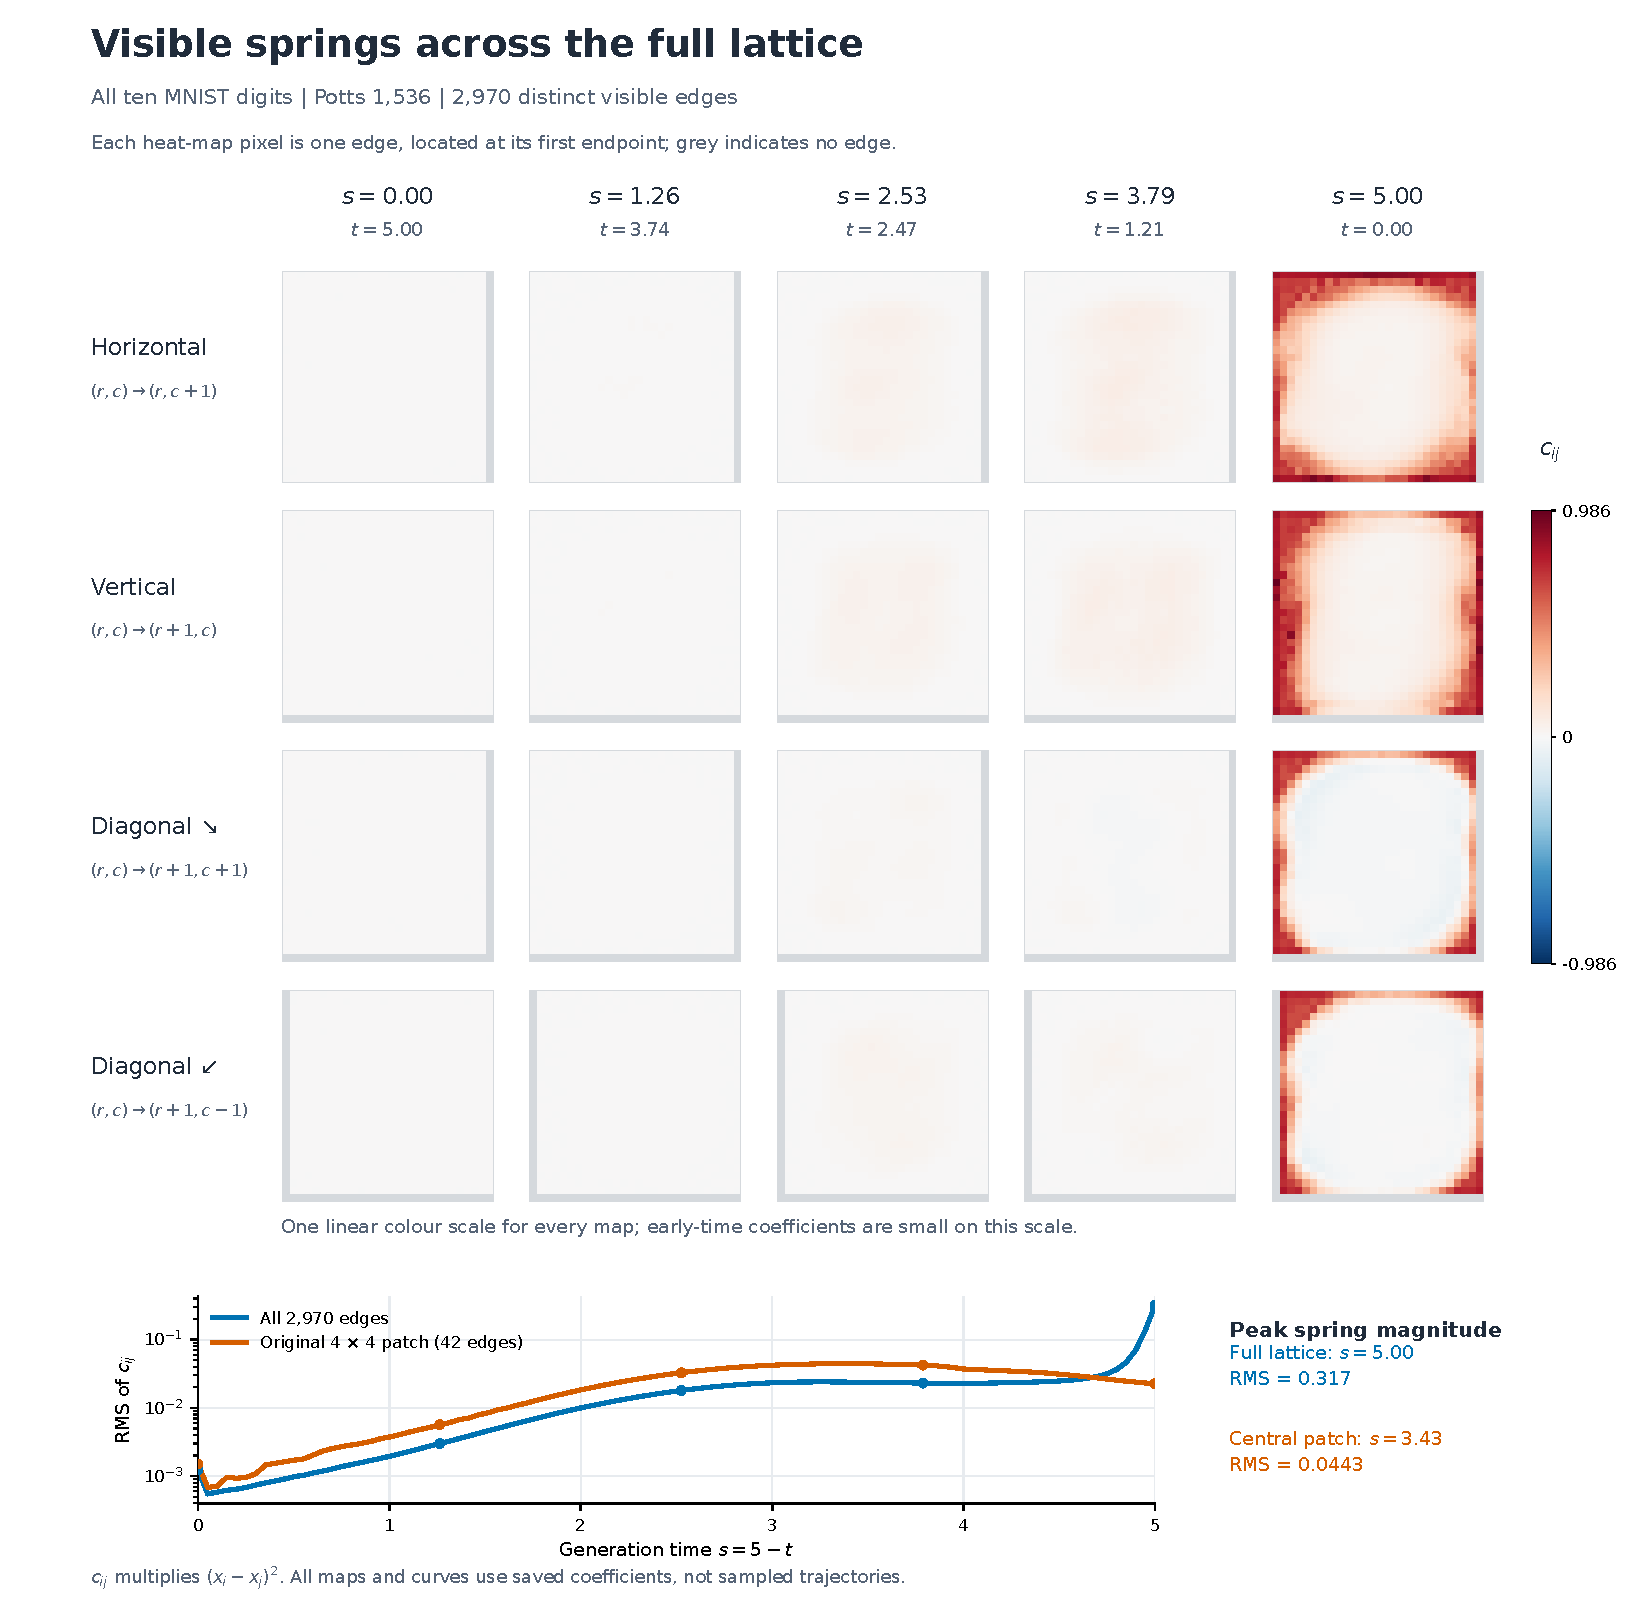
\includegraphics[trim={45 29.6 17 605},clip,width=.98\textwidth]{assets/visible_coupling_evolution.pdf}
  \vspace{.35cm}
  \begin{columns}[t,onlytextwidth]
    \column{.47\textwidth}\begin{block}{Central $4\times4$ patch}
      42 edges; peak at $s\simeq3.43$.\par The spring RMS decreases near the data end.
    \end{block}
    \column{.49\textwidth}\begin{block}{Full visible lattice}
      2970 edges; maximum at $s=5$.\par Strong boundary structure dominates the late rise.
    \end{block}
  \end{columns}
  \vspace{.2cm}\takeaway{Springs suppress differences between pixels. They do not, by themselves, fix the absolute background amplitude.}
  \note{This resolves the earlier impression that visible coupling is always largest at intermediate times. That is true for the chosen central patch, not for the global RMS. The full-lattice final RMS is 0.31698; the central patch peak is 0.04434. These are coefficient statistics, not force measurements along trajectories. Directional heat maps are in backup.}
\end{frame}

\begin{frame}{Visible-pair and global-Potts forces are comparable}
  \centering
  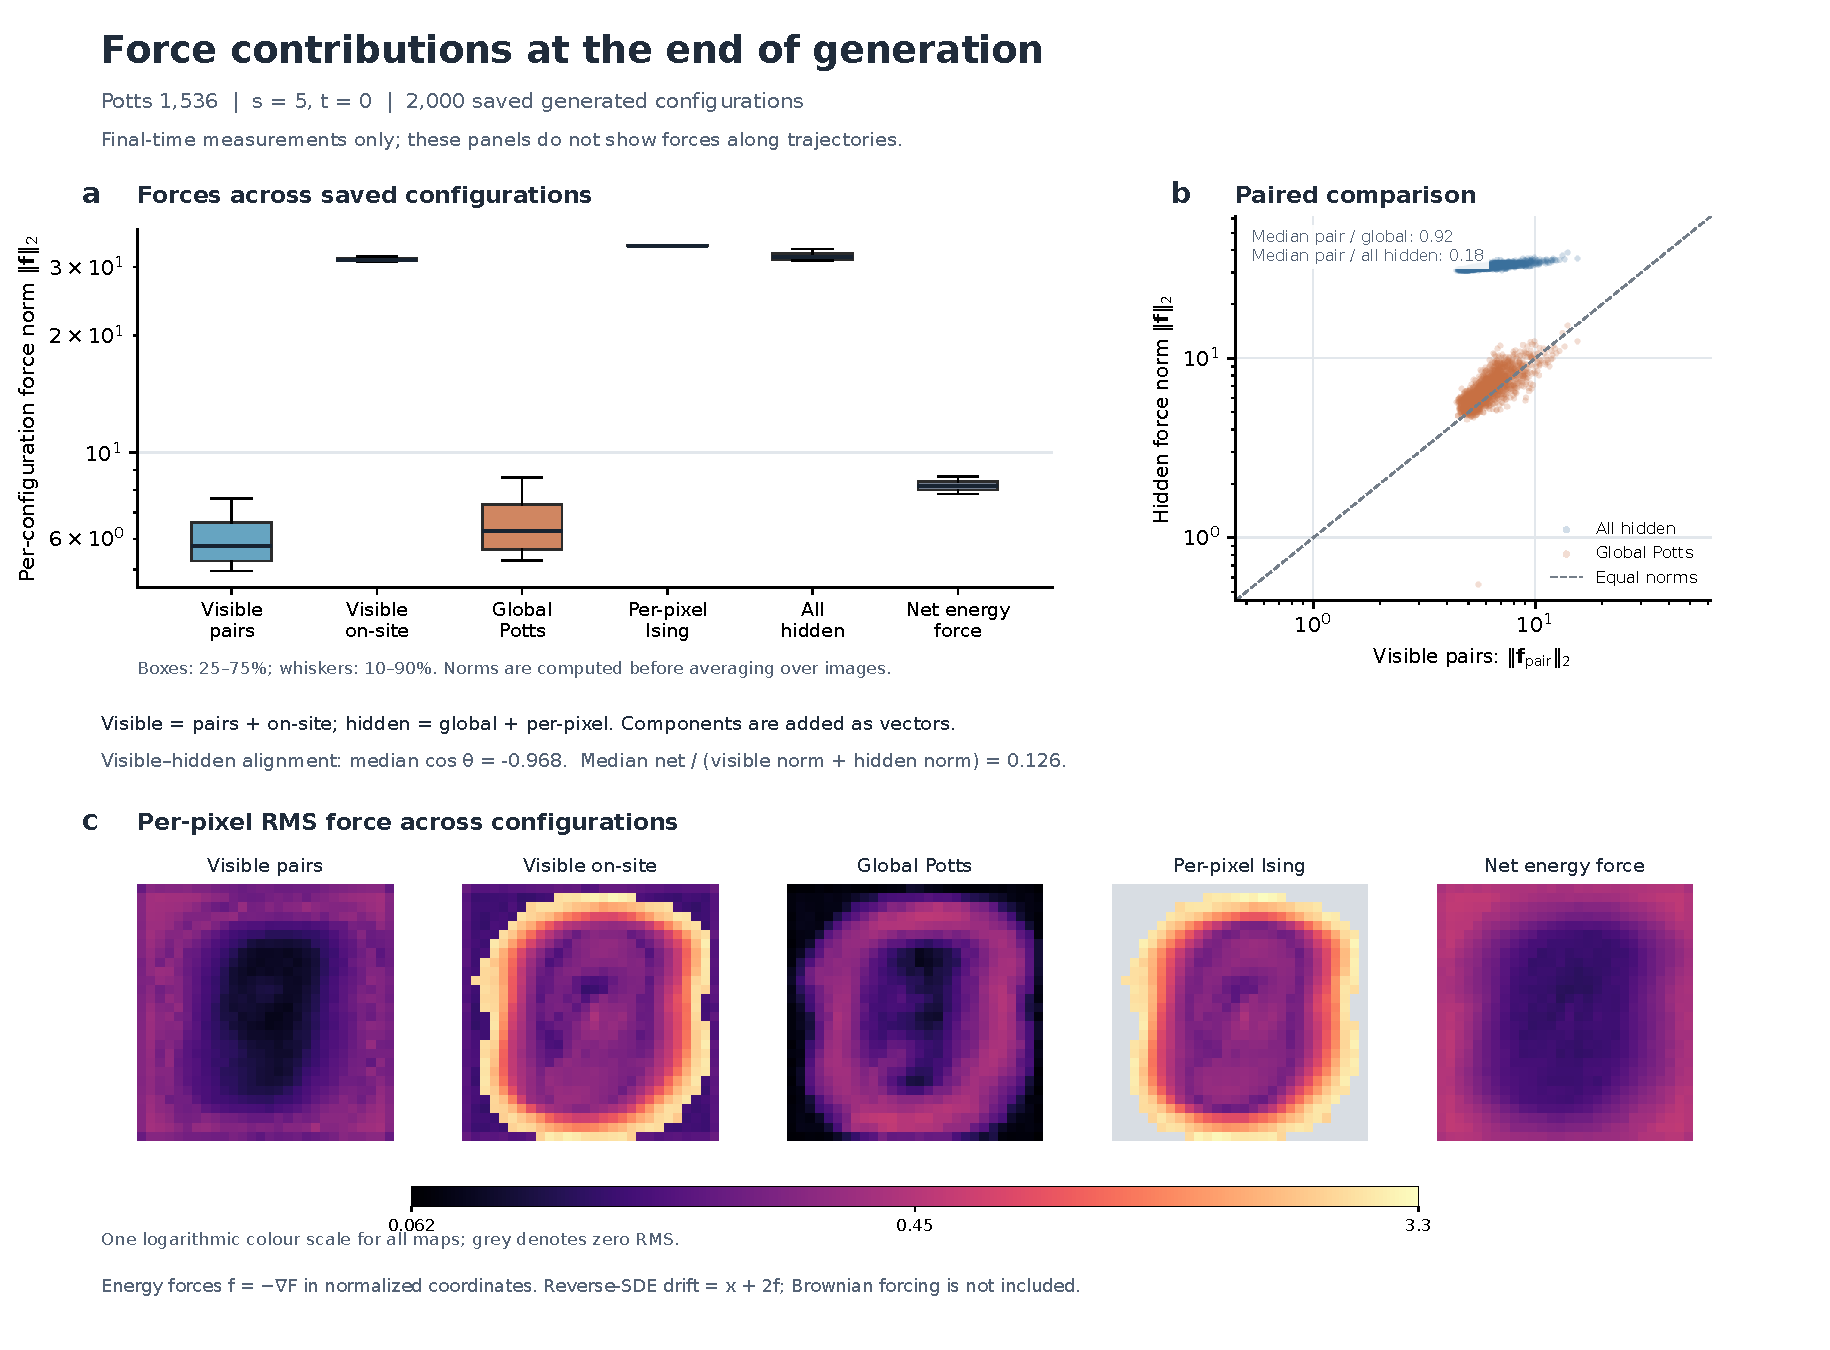
\includegraphics[trim={25 322 22.4 80},clip,width=.98\textwidth]{assets/force_comparison_final.pdf}
  \vspace{.15cm}
  \takeaway{Median norms: visible pairs $5.73$, global Potts $6.27$; on-site $31.30$, local Ising $34.01$.}
  \source{All 2000 saved final configurations, $s=5$; no quality filtering. Norms are calculated across pixels separately for each image.}
  \note{The forces are components of -grad F, not of the full drift x-2grad F. The left boxes show the distribution of per-configuration Euclidean norms. The right scatter compares paired measurements from each image; pair/global median ratio is 0.920. Total hidden force is a vector sum before taking its norm. This is not an ablation or proof of causal importance; force decomposition partly depends on the parameter gauge.}
\end{frame}

\begin{frame}{Large visible and hidden forces mostly oppose each other}
  \centering
  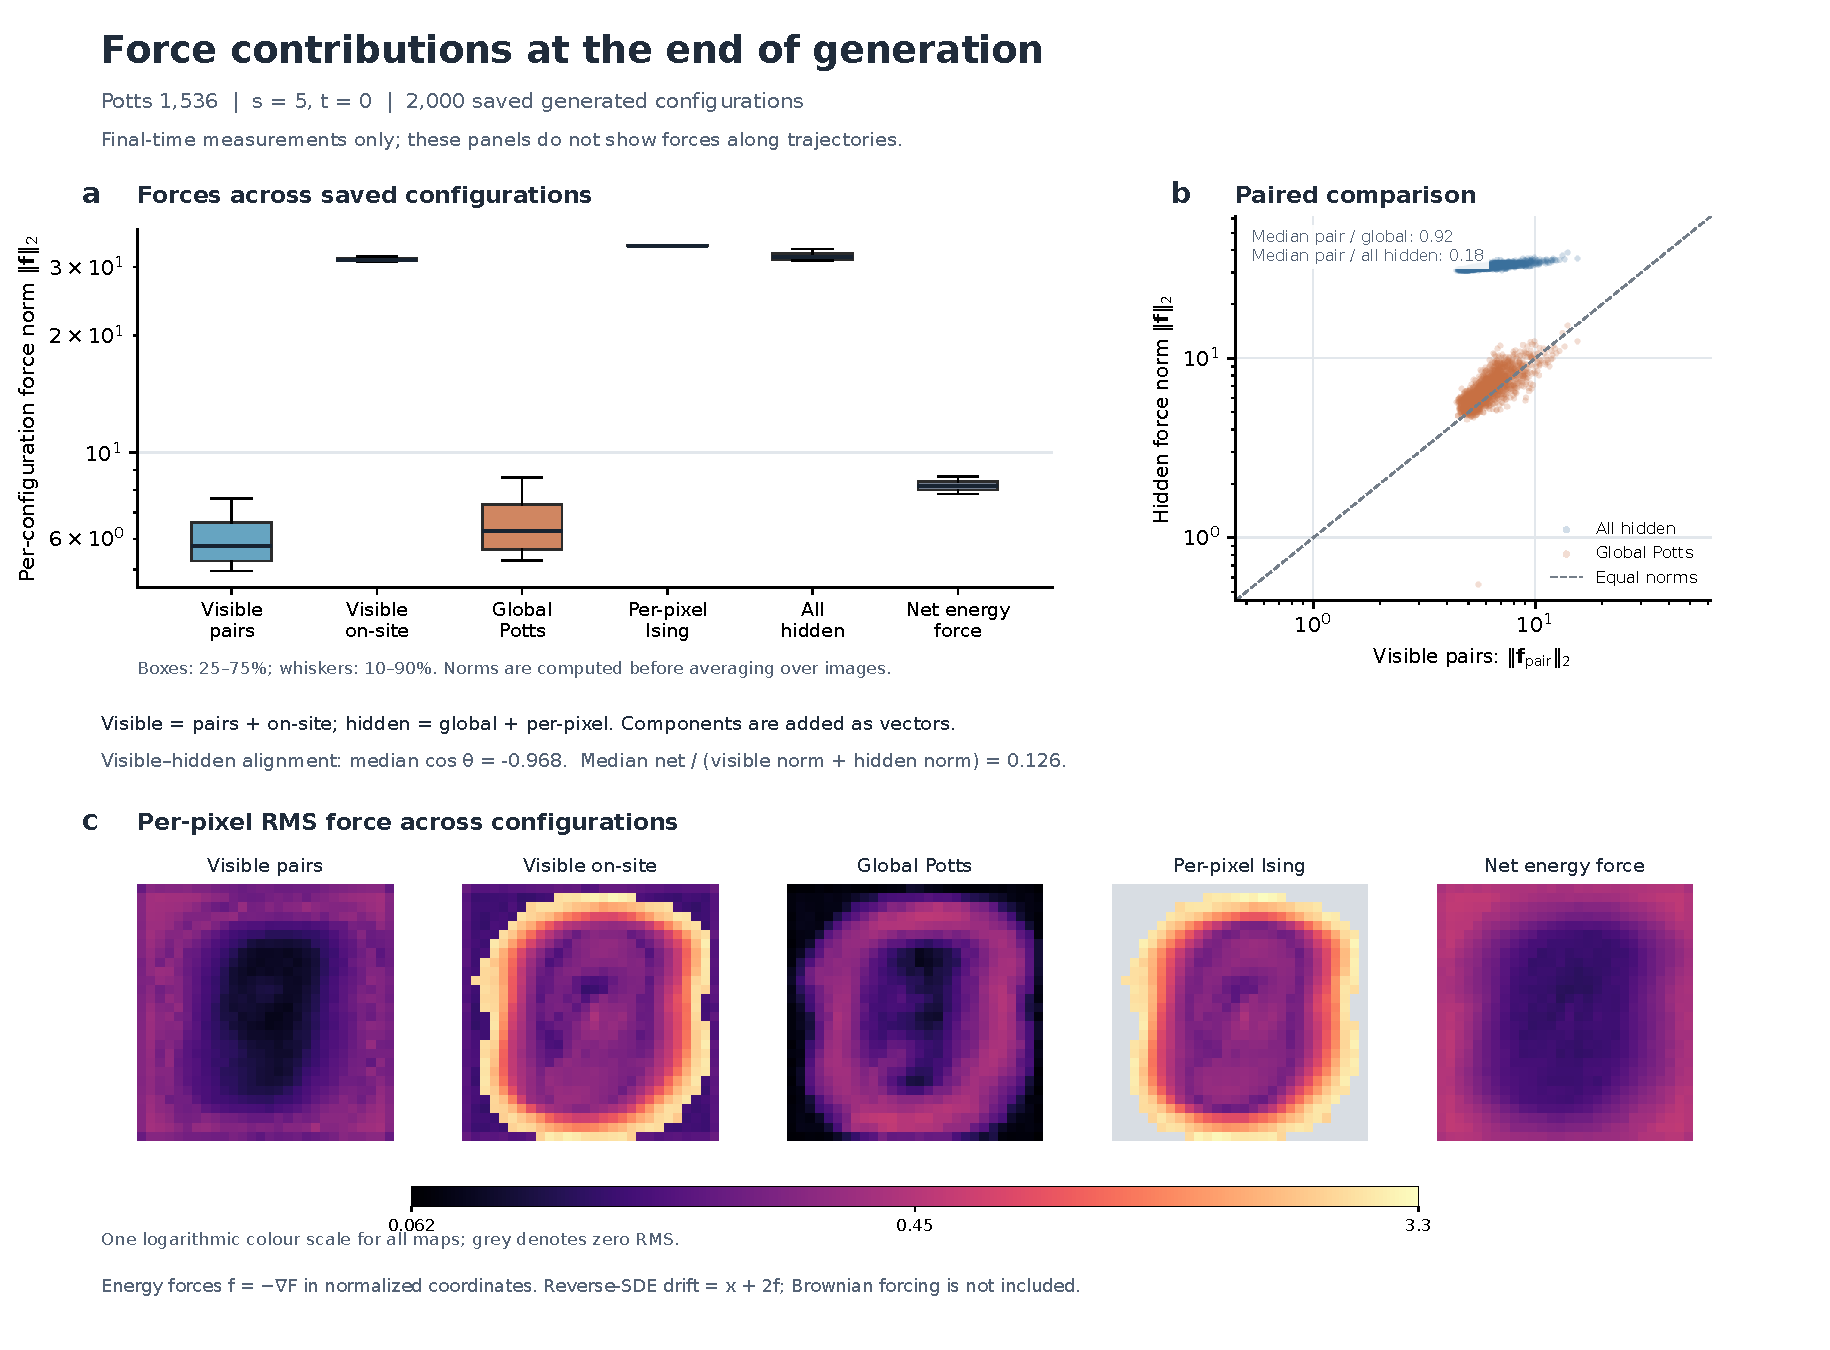
\includegraphics[trim={25 38 22.4 380},clip,width=.98\textwidth]{assets/force_comparison_final.pdf}
  \vspace{.25cm}
  \begin{columns}[c,onlytextwidth]
    \column{.48\textwidth}\begin{block}{Alignment}
      Median $\cos\angle(\bm f_{\rm vis},\bm f_{\rm hid})=-0.968$.
    \end{block}
    \column{.48\textwidth}\begin{block}{Cancellation}
      Median $\displaystyle\frac{\|\bm f_{\rm vis}+\bm f_{\rm hid}\|}{\|\bm f_{\rm vis}\|+\|\bm f_{\rm hid}\|}=0.126$.
    \end{block}
  \end{columns}
  \source{Spatial RMS across the same 2000 final configurations. Visible = pairs + on-site; hidden = global + local. One logarithmic colour scale.}
  \note{The strong cancellation is why comparing norms in isolation can mislead. It does not show that one component is dispensable. A common shift in all Potts W or Q can be compensated by visible bias or stiffness without changing the total free energy, moving force between the on-site/global-hidden contributions. The net force is the invariant quantity. These data concern the final time only.}
\end{frame}

\begin{frame}{Movie: one visible trajectory and its Potts probabilities}
  \centering
  \includegraphics[height=5.45cm]{assets/movie_poster.png}\par\vspace{.08cm}
  \textattachfile[mimetype=video/mp4,description={Potts state probabilities, 20 second MP4},color=0 0.49 0.57]{media/potts-state-probabilities.mp4}{\beamergotobutton{Open attached MP4}}
  \hspace{.5cm}\href{run:media/potts-state-probabilities.mp4}{\beamergotobutton{Open companion MP4}}
  \source{20 seconds; 397 saved frames. One actual reverse-SDE trajectory. Curves show conditional probabilities, not simulated hidden jumps.}
  \note{Pause the presentation and play the 20-second movie. PDF attachment support varies by viewer; the MP4 is also supplied separately in media/. The trajectory reproduces saved sample 0 of the base-2000 set: final maximum absolute amplitude discrepancy is 2.76e-5 due to restarting the adaptive solver at parameter knots. Posterior normalization error is below 5e-16. Group labels are initial cluster majority labels. The movie displays visible image, initial digit-group probability, fixed competing states, and between/within-group entropy. No new training was needed.}
\end{frame}

\begin{frame}{State confidence concentrates before the digit is clear}
  \centering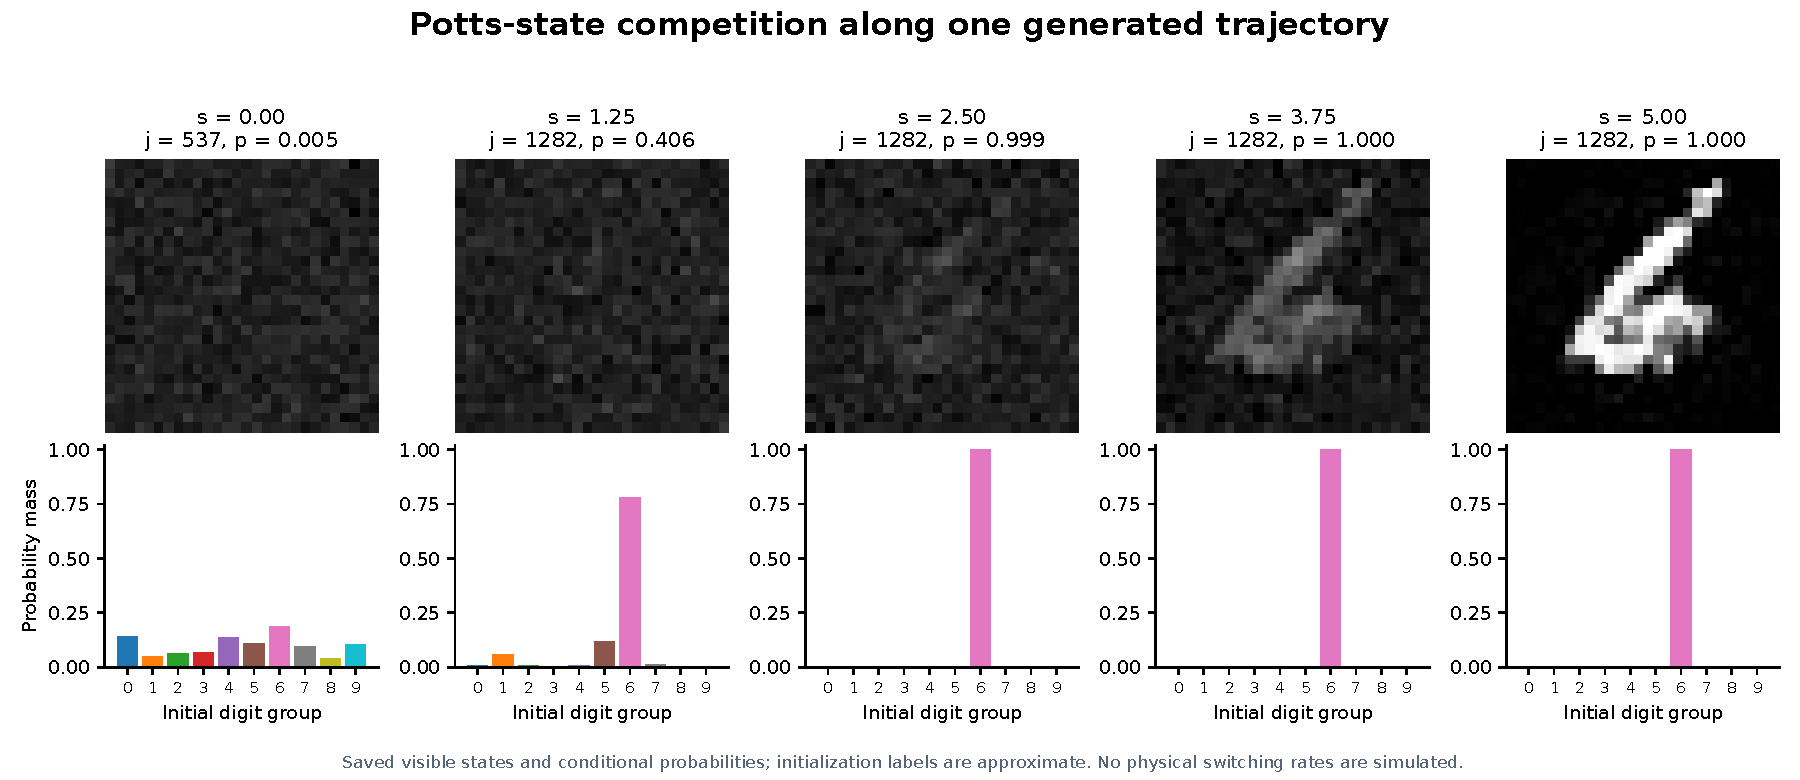
\includegraphics[trim={0 20 0 32},clip,width=.98\textwidth]{assets/potts_video_summary.pdf}
  \vspace{.2cm}
  \takeaway{In this trajectory: group confidence exceeds $90\%$ from $s\simeq1.65$; individual-state confidence from $s\simeq1.94$.}
  \source{Thresholds remain exceeded at all subsequent saved frames. Final state 1282 has initial group 6. One illustrative trajectory, not a population study.}
  \note{The most probable individual state initially changes among groups and later among several states associated with 6. Aggregate competition across groups is still appreciable around s=1.5. The final state becomes the persistent argmax around s=1.06 while its probability is only about 0.21, so argmax stability alone is not commitment. Final group 6 confidence crosses and remains over 90 percent around1.65; individual state confidence does so around1.94. Avoid presenting these timings as universal. The visible digit emerges more clearly later.}
\end{frame}

\begin{frame}{What is established, and what should come next?}
  \begin{columns}[t,onlytextwidth]
    \column{.48\textwidth}
      \begin{block}{Established numerically}
        \begin{itemize}\setlength\itemsep{.25cm}
          \item Trainable visible and hidden energy parameters.
          \item All-ten-digit generation in the conditional-mean model.
          \item Structured coupling schedules and interpretable force contributions.
        \end{itemize}
      \end{block}
    \column{.48\textwidth}
      \begin{block}{Follow-up directions}
        \begin{itemize}\setlength\itemsep{.25cm}
          \item Explicit hidden dynamics and finite switching rates.
          \item Finite-read learning and architectural ablations.
          \item Scaling, encoder/decoder interfaces and hardware constraints.
        \end{itemize}
      \end{block}
  \end{columns}
  \vspace{.35cm}\takeaway{Proposed paper focus: local training and a working latent extension. Treat physical kinetics and scaling as follow-up studies.}
  \note{This is a proposed framing for discussion with the PI, not a claim that scaling questions are resolved or that a journal will accept this scope. The key boundary is that current generation assumes fast conditional equilibration and current ten-digit training uses exact hidden statistics. Controlled ablations would be needed to quantify the necessity of local Ising units, visible interactions, or particular hidden couplings. The current results support a demonstration, not a hardware efficiency advantage.}
\end{frame}

\appendix
\begin{frame}{Backup: the Gaussian special case}
  If the common energy is quadratic,
  \[G(\vx)=\tfrac12\vx^T A\vx+\bm\ell^T\vx,
  \qquad a_m=b_m+\bm W_m^T\vx+\bm Q_m^T\vx^2,\]
  define $H_m=A-2\operatorname{diag}(\bm Q_m)$. For $H_m\succ0$,
  \[\boxed{p(\vx\mid m)=\mathcal N(\bm\mu_m,\Sigma_m),\quad
    \bm\mu_m=H_m^{-1}(\bm W_m-\bm\ell),\quad\Sigma_m=T H_m^{-1}.}\]
  \vspace{.2cm}
  \begin{itemize}\setlength\itemsep{.15cm}
    \item $Q_m$ changes precision/stiffness; visible springs also affect covariance.
    \item $W_m$ sets the linear tilt; $b_m$ cancels from normalized $p(\vx\mid m)$.
    \item Mixture weights also depend on each component's normalization.
  \end{itemize}
  \vspace{.2cm}\takeaway{The actual quartic-plus-local-Ising model is more general than this Gaussian special case.}
  \note{Completing the square gives mixture weights proportional to $\det(H_m)^{-1/2}\exp[(b_m+\tfrac12\bm h_m^T H_m^{-1}\bm h_m)/T]$, where $\bm h_m=\bm W_m-\bm\ell$. They are not simply softmax$(b/T)$. The positivity condition matters: $Q$ is not constrained to define a standalone Gaussian. In the actual model quartic confinement remains present.}
\end{frame}

\begin{frame}{Backup: state 1, initially associated with digit 6}
  \statefigure{1}{566.4}{140}
  \note{Full saved W and Q evolution for state1. This is the same source figure and scale as state0, with time headings restored after cropping.}
\end{frame}
\begin{frame}{Backup: state 2, initially associated with digit 2}
  \statefigure{2}{304.4}{402}
  \note{Full saved W and Q evolution for state2. Initial digit association is not a measurement of final class purity.}
\end{frame}
\begin{frame}{Backup: state 4, initially associated with digit 9}
  \statefigure{4}{41.4}{664}
  \note{Full saved W and Q evolution for state4. All colours share coefficient-family scales across the four selected states and all five times.}
\end{frame}

\begin{frame}{Backup: signed horizontal and vertical spring maps}
  \begin{columns}[c,onlytextwidth]
    \column{.9\textwidth}\centering
      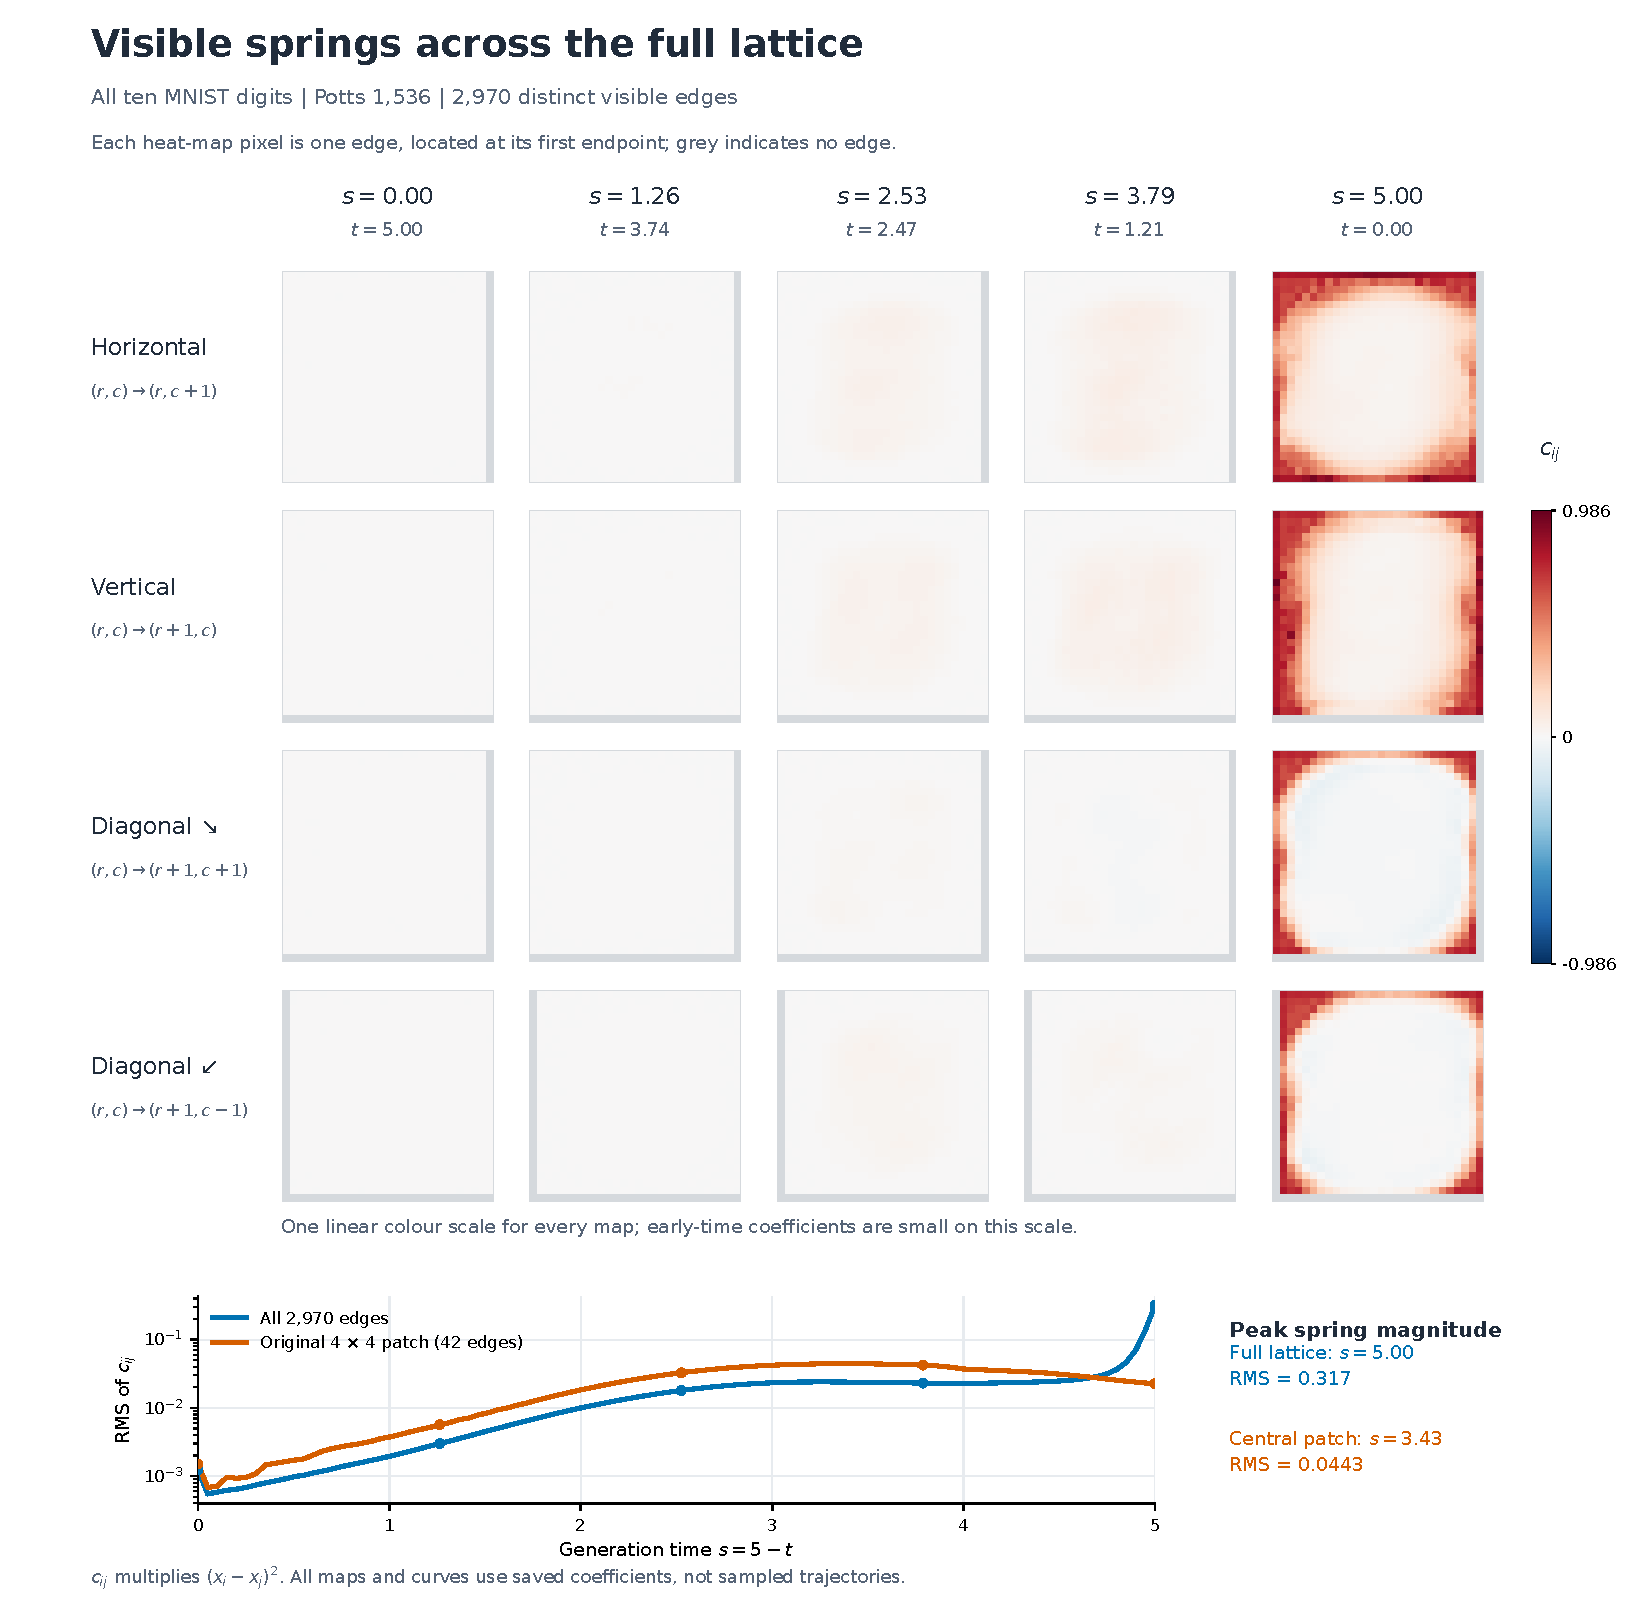
\includegraphics[trim={30 425 68 82},clip,width=\linewidth]{assets/visible_coupling_evolution.pdf}
    \column{.08\textwidth}\centering
      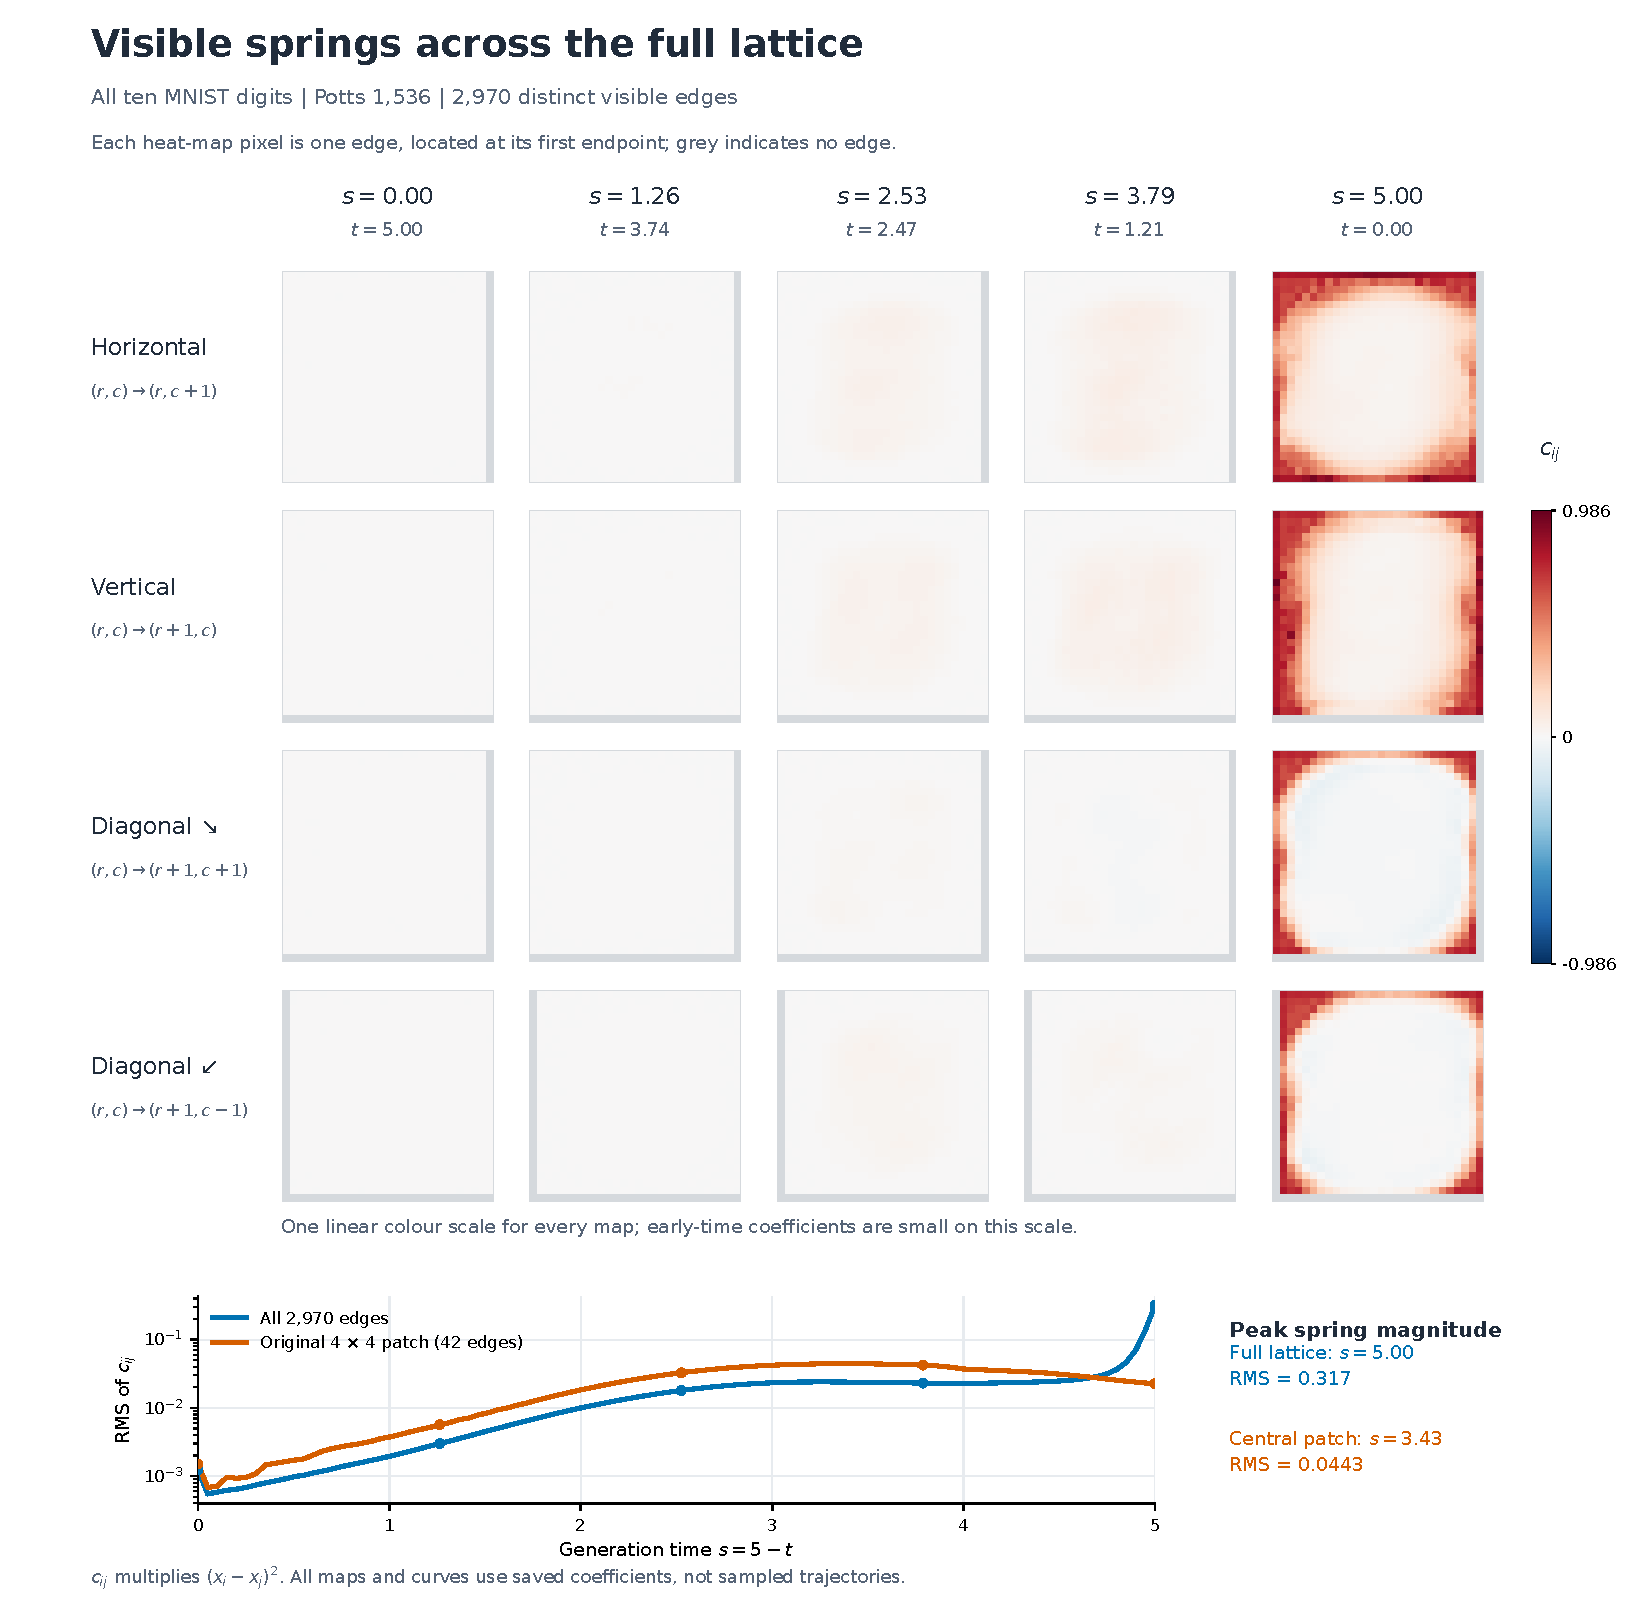
\includegraphics[trim={728 307.6 11 205},clip,width=.8\linewidth]{assets/visible_coupling_evolution.pdf}
  \end{columns}
  \vspace{.2cm}\takeaway{Each map location represents one edge. A shared linear colour scale makes weak early couplings look nearly white.}
  \note{These maps preserve edge orientation and sign, unlike the incident RMS maps. Grey denotes absence of that edge. Each undirected edge is represented exactly once across the four orientations. The common scale is shared across all directions and times.}
\end{frame}
\begin{frame}{Backup: signed diagonal spring maps}
  \begin{columns}[c,onlytextwidth]
    \column{.9\textwidth}
      \noindent\hspace*{.1394\linewidth}\makebox[.17118\linewidth]{$s=0$}\makebox[.17118\linewidth]{$1.26$}\makebox[.17118\linewidth]{$2.53$}\makebox[.17118\linewidth]{$3.79$}\makebox[.17118\linewidth]{$5$}\par\vspace{.06cm}
      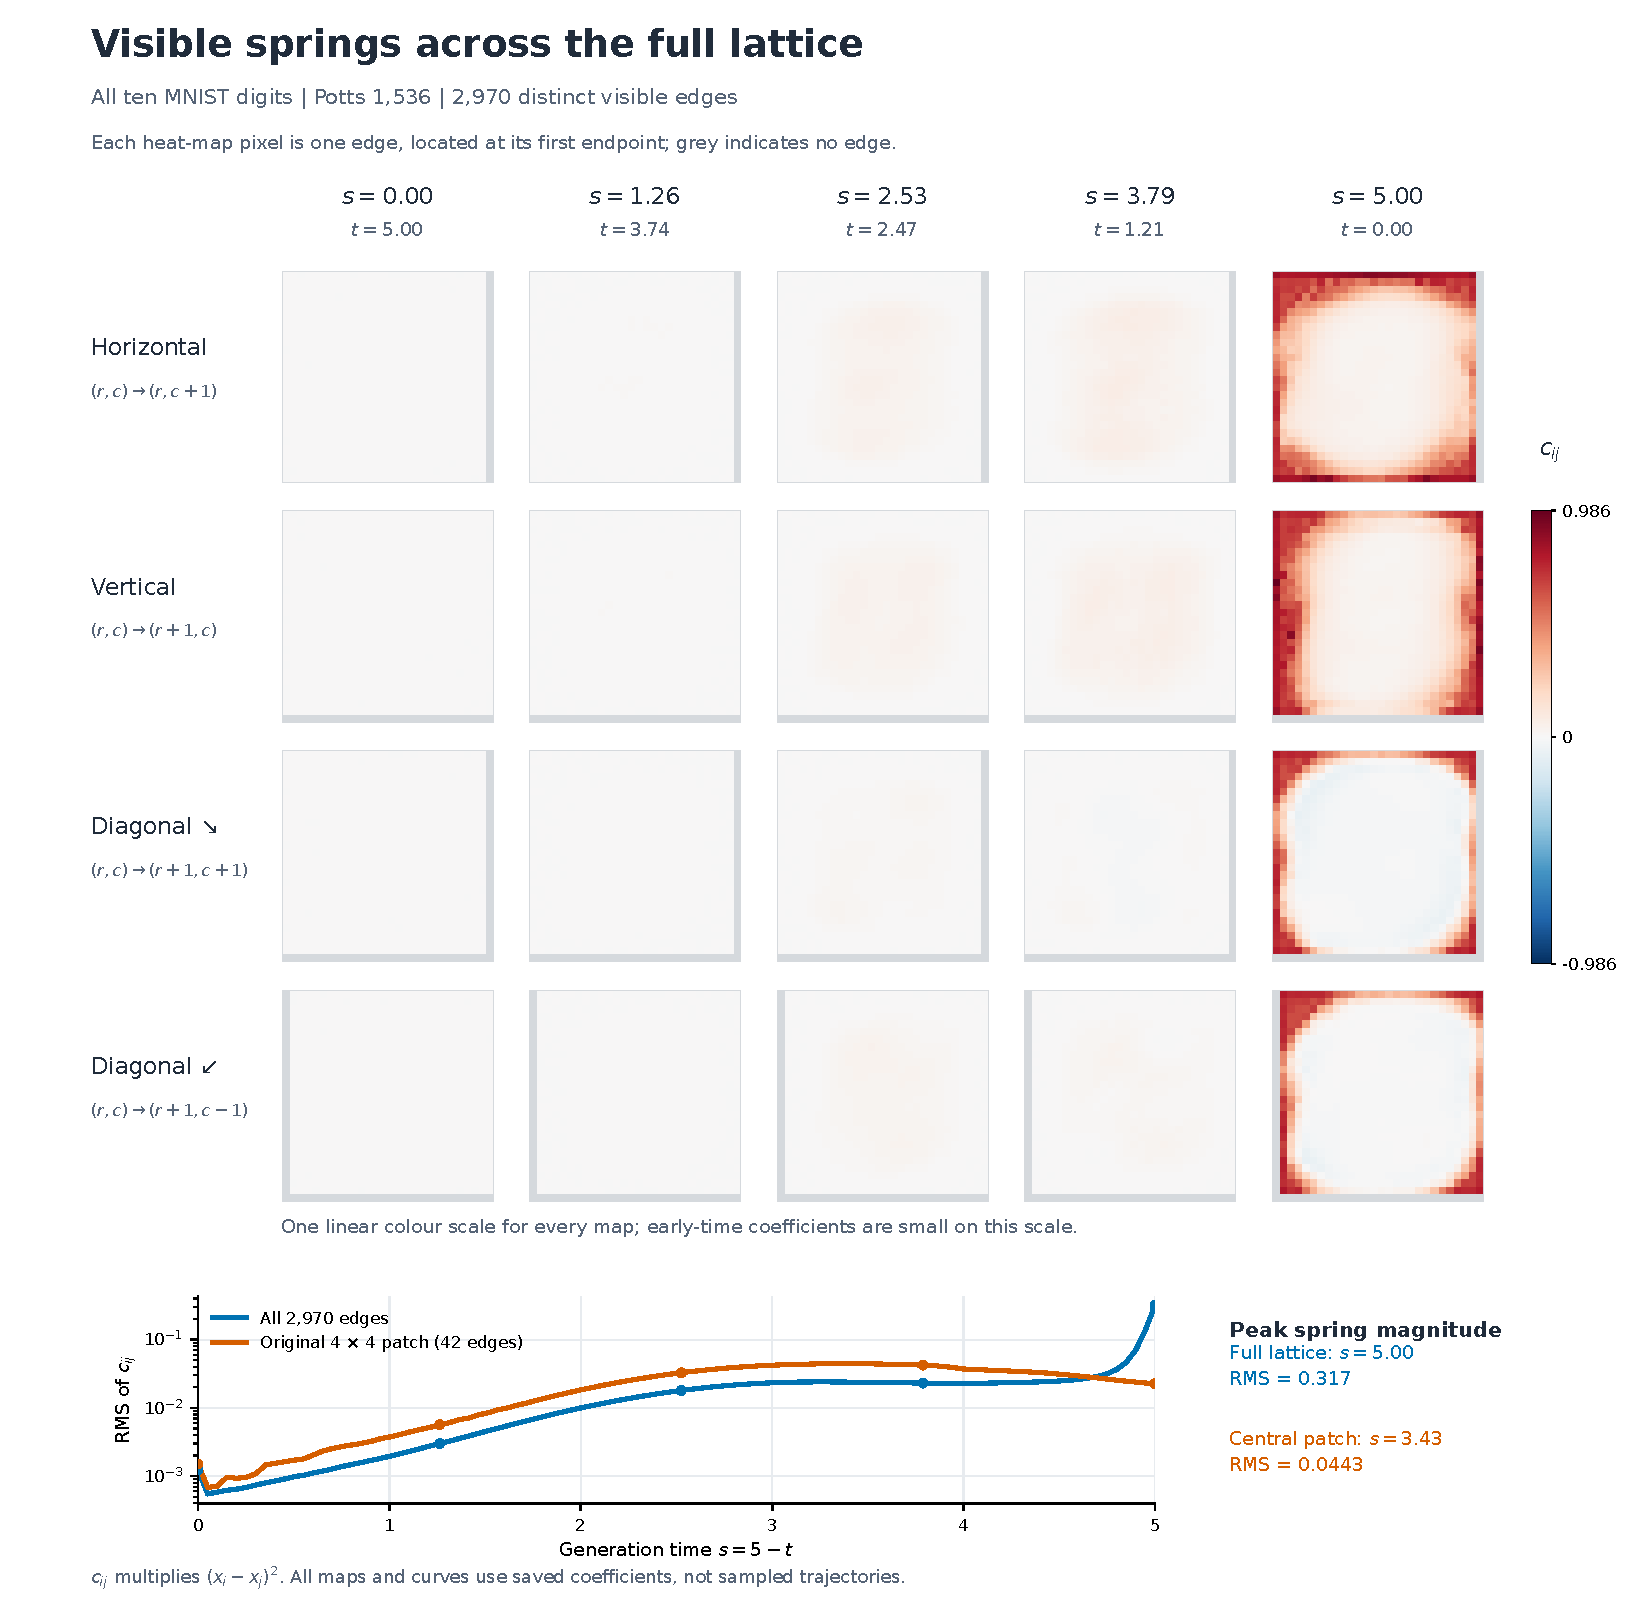
\includegraphics[trim={30 196.6 68 354},clip,width=\linewidth]{assets/visible_coupling_evolution.pdf}
    \column{.08\textwidth}\centering
      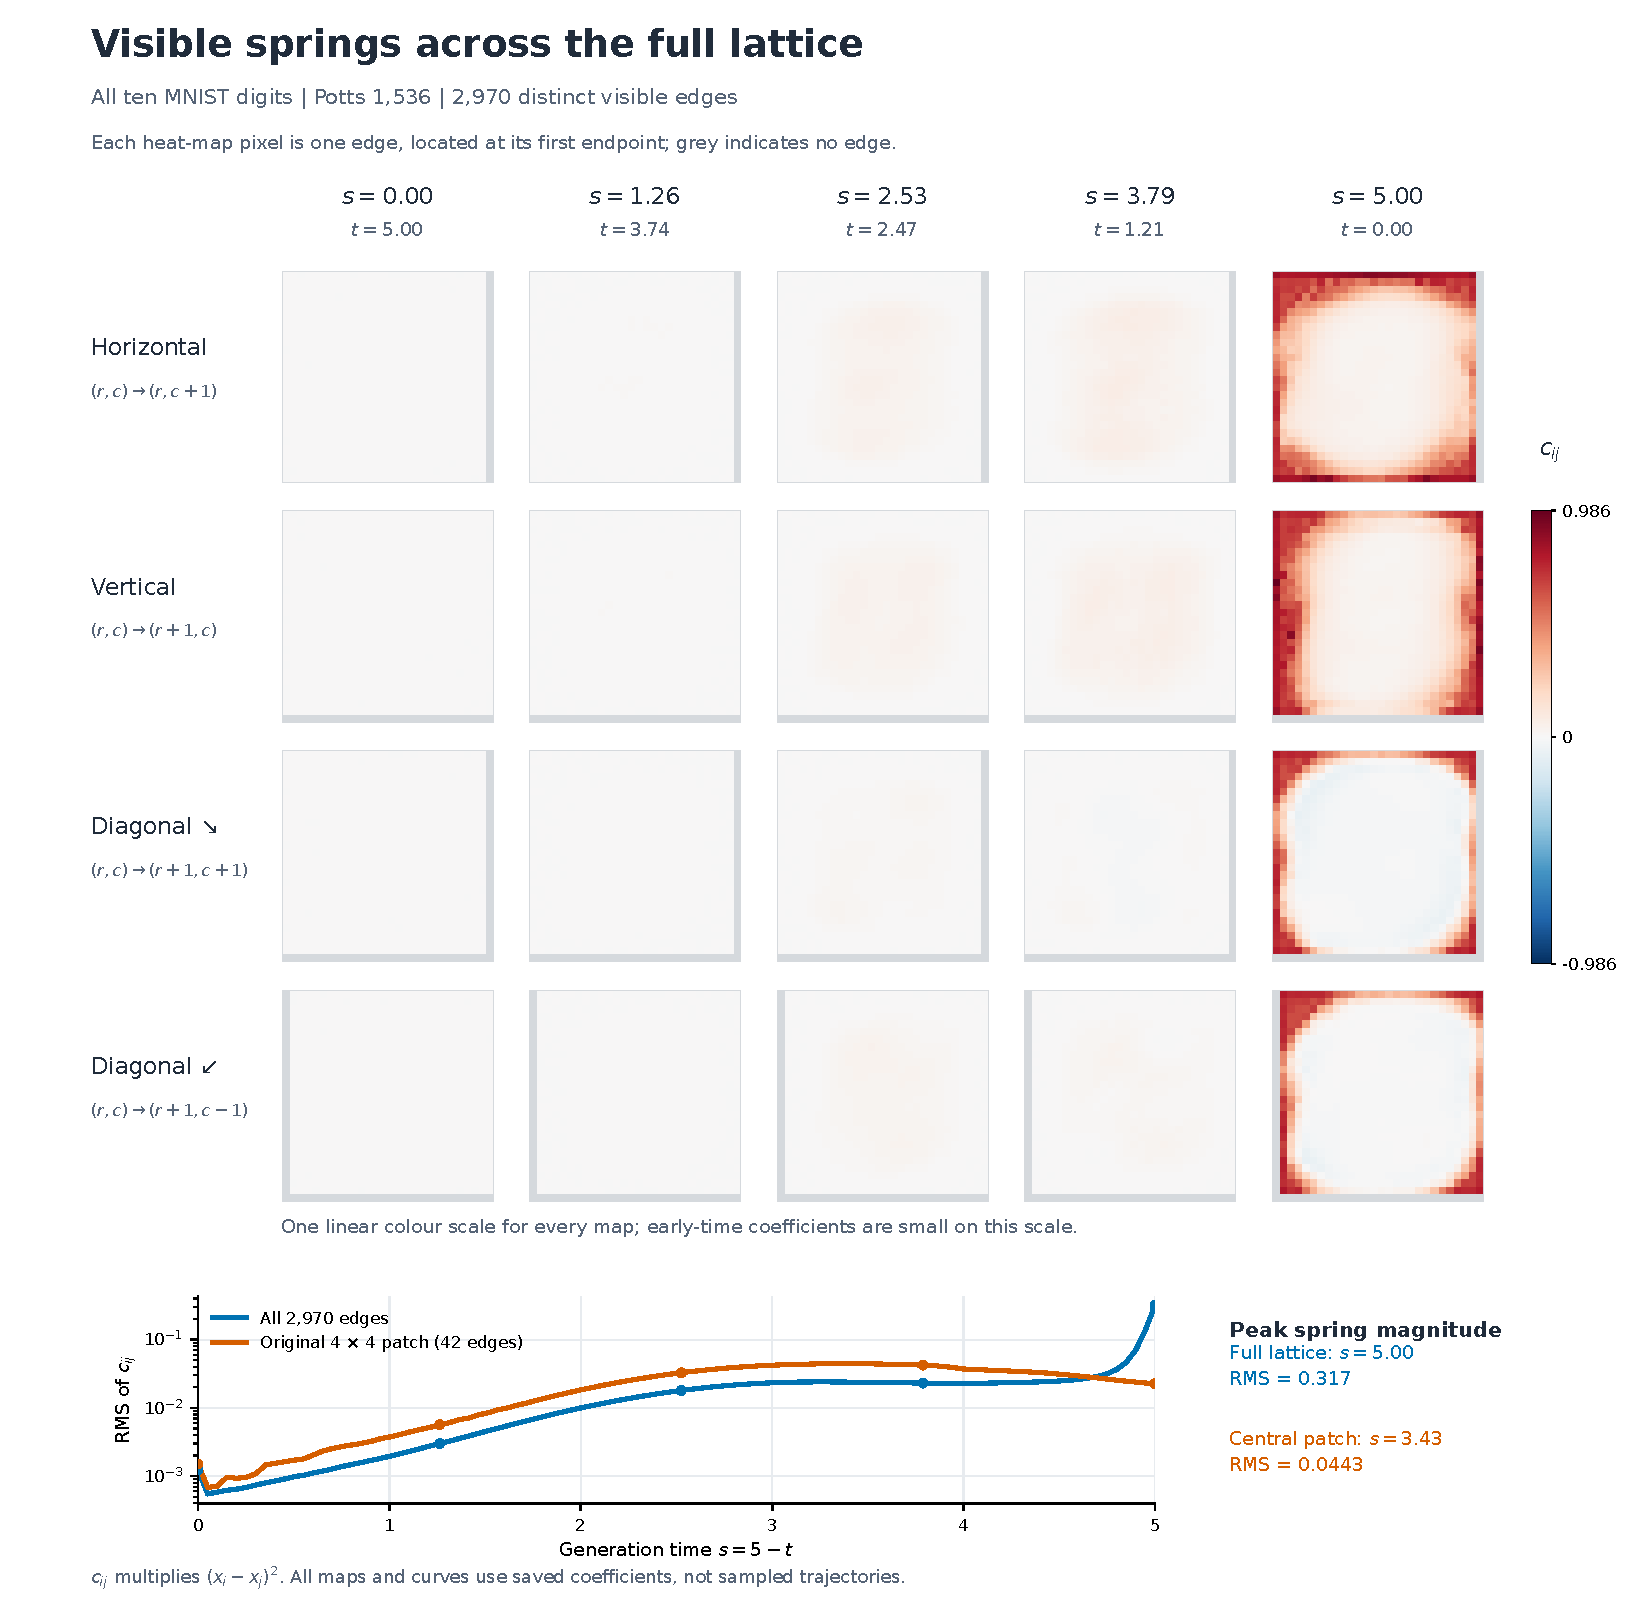
\includegraphics[trim={728 307.6 11 205},clip,width=.8\linewidth]{assets/visible_coupling_evolution.pdf}
  \end{columns}
  \vspace{.2cm}\takeaway{Diagonal edges complete the eight-neighbour lattice; boundary pixels have fewer neighbours.}
  \note{The restored headings use generation time s=0,1.26,2.53,3.79,5. These are saved coefficient maps rather than sampled forces.}
\end{frame}

\end{document}
